% !TeX spellcheck = sv_SE
\documentclass[a4paper, 12pt]{report}

\usepackage[swedish]{babel}
\usepackage[T1]{fontenc}
\usepackage{lmodern}
\usepackage[utf8]{inputenc}

\usepackage{amsmath}
\usepackage{amssymb}
\usepackage{amsfonts}
\usepackage{amsthm}

\usepackage{icomma}

\usepackage{graphicx}

\usepackage{enumitem}

\DeclareMathOperator{\sign}{sign}

\theoremstyle{definition}
\newtheorem{thm}{Sats}[section]
\newtheorem{lem}[thm]{Lemma}
\newtheorem{cor}[thm]{Korollarium}
\newtheorem{defi}{Definition}[section]
\newtheorem{ex}{Exempel}[section]
\theoremstyle{remark}
\newtheorem*{rem}{Observation}

\newtheorem*{reas}{Orsak}

\newcommand{\bfbeta}{{\boldsymbol{\beta}}}
\renewcommand\qedsymbol{$\blacksquare$}

\newcommand{\bfx}{\mathbf{x}}

\newcommand{\bfy}{\mathbf{y}}

\newcommand{\llangle}{\left\langle}
\newcommand{\rrangle}{\right\rangle}

\newcommand{\sephyp}{\{ \mathbf{x} : f\left(\mathbf{x}\right)=\inner{\bfx}{\bfbeta}_\mathcal{H} + \beta_0=0\}}

\newcommand{\entsephyp}{\{ \mathbf{x} : f\left(\mathbf{x}\right)=\mathbf{x}^\intercal \bfbeta + \beta_0=0,~y_if\left(\mathbf{x}_i\right)\geq0,~i=1,\dots,~N,~\left\|\bfbeta\right\|=1\}}

\newcommand{\inprod}[2]{\llangle \mathbf{#1}, \mathbf{#2}\rrangle}

\newcommand{\inner}[2]{\llangle #1, #2 \rrangle}

\newcommand{\hil}{\mathcal{H}}

\interfootnotelinepenalty=10000

\title{{\Huge Stödvektormaskiner}\\
{\Large Linjära hyperplan i Hilbertrum}\\
~\\
{\large Kandidatavhandling i matematik}\\
{\large Fakulteten för naturvetenskaper och teknik}\\
{\large Åbo Akademi}}
\author{{\Large Oscar Granlund}\\
{\Large37920}\\
\\
{\large Handledare:}\\{\large Anne-Maria Ernvall-Hytönen}}
\date{31 oktober 2018}


\begin{document}
\maketitle

\begin{abstract}
	Stödvektormaskinen (SVM) är en metod för att klassificera observationer som var mycket populär under den senare delen av 90-talet och början av 00-talet.
	Metoden går ut på att man passar in ett hyperplan mellan observationernas klasser och använder hyperplanet som gräns för övergången mellan klasserna.
	I denna avhandling undersöks och härleds metoden med start i ett enkelt optimeringsproblem som i tre steg görs mera allmänt.
	Först undersöks ett optimeringsproblem som kräver att alla observationer går att klassificera rätt, speciellt läggs vikt på att med Lagrangemultiplikatorer karaktärisera den optimala lösningen.
	Till näst undersöks några varianter av det första optimeringsproblemet där man tillåter att observationerna klassificeras fel, igen karaktäriseras den optimala lösningen.
	Till sist presenteras en introduktion till teorin om Hilbertrum med reproducerande kärnor som ger ett sätt att generalisera de hittills linjära klassificeringsmetoderna (samt andra linjära metoder) till en olinjär klassificeringsmetod.
%	I denna avhandling presenteras stödvektormaskiner (SVM) med fokus på att noggrant förklara motiveringarna bakom de steg som oftast presenteras i introduktionslitteraturen, både för den ursprungliga algoritmen med hårda marginaler och algoritmen med mjuka marginaler. Speciellt läggs vikt på analys av lösningen som karaktäriseras med hjälp av Lagrangemultiplikatorer. Till sist presenteras också en introduktion till teorin för Hilbertrum med reproducerande kärnor där huvudresultatet är verifieringen av att den funktion som vanligtvis presenteras som inreprodukt uppfyller kraven för inreprodukter. Som följd visas att varje symmetrisk positivt semidefinit funktion $k\left(\bfx, \bfy\right)$ kan ses som en inreprodukt i något rum.
\end{abstract}

\tableofcontents

\chapter{Inledning}
Tack vare en ökande beräkningsförmåga samt användbarhet hos datorer under senare delen av 1900-talet forskades det flitigt om hur man bäst använder datorer för beräkning och lösning av statistiska metoder och problem.
I samband med detta uppstod även forskningsområdet maskininlärning där tyngdpunkten låg mera på datorerna.
En tidig algoritm var Frank Rosenblatts \emph{Perceptron} (år 1957) \cite{Rosenblatt} där man med inspiration från hjärnans neuroner försökt klassificera \emph{observationer} $\mathbf{x}$ genom att dra ett \emph{hyperplan} mellan klasserna.
År 1963 gav Aleksandr Lerner och Vladimir Vapnik en variant av Rosenblatts perceptron där \emph{optimala separerande hyperplan} används för att klassificera observationerna \cite{VapnikLerner1963}.
Lerner och Vapniks algoritm är matematiskt mera tilltalande än Rosenblatts eftersom den optimala lösningen kan visas vara unik, men det finns fortfarande några problem, bland annat går algoritmen bara att använda om observationsparen är \emph{linjärt separabla}.
År 1968 föreslog Fred Smith \cite{Smith} en generaliserad algoritm som använde \emph{slackvariabler} för att även fungera för icke linjärt separabla observationspar.
Smiths arbete med slackvariabler undersöktes vidare av Kristin Bennet och Olvi Mangasarian år 1992 \cite{BennetMangasarian}.

Parallellt med forskningen i de linjära optimalt separerande hyperplanen forskades det om tillämpningar av funktioner kallade \emph{kärnor}, med avstamp i James Mercers forskning (1909) i \emph{positiva} funktioner \cite{Mercer} och Nachman Aronszajns fortsatta forskning (1950) om \emph{reproducerande} kärnor \cite{Aronszajn}.
Kärnor föreslogs av Mark Aizerman, Emmanuil Braverman och Lev Rozonoer \cite{Aizerman} för att generalisera perceptron-algoritmen till en algoritm för olinjär klassificering.
Efter att kärnorna visades vara nyttiga för andra algoritmer, se till exempel Grace Wahbas bok om spline-modeller (1990) \cite{Grace} tillämpades kärnor även på den ursprungliga algoritmen med optimalt separerande hyperplan av Bernhard Boser, Isabelle Gyuon och Vladimir Vapnik i 1992 \cite{BoserGyuonVapnik}.
Snart därefter generaliserades även Bennets och Mangasarians algoritm av Corinna Cortes och Vladimir Vapnik i 1995 \cite{CortesVapnik}, detta är algoritmen som vanligtvis associeras med begreppet \emph{stödvektormaskin} (Support Vector Machine, SVM) och därmed är det den jag vill härleda.

I avhandlingen kommer till först den ursprungliga algoritmen att undersökas för att sedan modifieras med slackvariabler, upplägget följer långt Trevor Hasties, Robert Tibshiranis och Jerome Friedmans bok \cite{ESL}, speciellt kapitlet om optimalt separerande hyperplan samt den mjuka utvidgningen med slackvariabler.
Därefter kommer de reproducerande kärnorna att undersökas, för det följs i stora drag Bernhard Schölkopfs och Alexander Smolas bok \cite{LearningKernels}.

Precis som många andra metoder inom statistiken och maskininlärningen bygger stödvektormaskinen på ett konvext optimeringsproblem och på grund av detta borde läsaren vara bekant med koncept ur konvex optimering.
En bra introduktion är Stephen Boyd och Lieven Vandenberghes bok \cite{Boyd}.
Främst kommer teorin om kvadratiska optimeringsproblem och analys av duala problem med hjälp av Lagrangemultiplikatorer att användas.

%\chapter{Stödvektormaskiner (SVM)}

\chapter{Hilbertrumteori}\label{chap:hilbert}

\section{Geometrisk begrepp}
I många statistiska metoder används enkla geometriska koncept, till exempel plan eller linjer, för att dra slutsatser angående insamlat data.
Ofta vill man även hitta den bästa modellen, till exempel den modell som minimerar avståndet mellan observationerna och modellens predikterade värden (tänk som i linjär regression) eller den modell som maximerar det minsta avståndet mellan två klasser.
För att effektivt kunna resonera om hur rummet man arbetar i ser ut visar det sig att teorin om \emph{inreproduktrum}, eller närmare bestämt \emph{Hilbertrum}, ger många bra verktyg.
Ett \emph{Hilbertrum}, $\mathcal{H}$, är ett vektorrum $X$ försett med en \emph{inreprodukt}, $\llangle \cdot, \cdot\rrangle$, som dessutom är \emph{fullständigt}.

\begin{defi}[Enligt \cite{Young}]\label{def:inreprodukt}
	Låt $X$ vara ett vektorrum. En \emph{inreprodukt} är en funktion $\langle \cdot , \cdot \rangle: X\times X \longmapsto \mathbb{R}$ sådan att, för alla $\mathbf{x},~\mathbf{y},~\mathbf{z}\in X$ och alla $\lambda \in \mathbb{R}$, gäller:
	\begin{enumerate}[label=\textbf{IP\arabic*}]
		\item \label{IP1} $\inprod{x}{y} = \inprod{y}{x}$,
		\item \label{IP2} $\langle \lambda \mathbf{x}, \mathbf{y}\rangle = \lambda \inprod{x}{y}$,
		\item \label{IP3} $\inprod{x+y}{z} =\inprod{x}{z} + \inprod{y}{z}$,
		\item \label{IP4} $\inprod{x}{x} \geq 0$ där likhet gäller om och endast om $\mathbf{x} = \mathbf{0}$. 
	\end{enumerate}
\end{defi}

\begin{defi}\label{def:Cfull}
	Ett inreproduktrum $X$ är \emph{fullständigt} om varje Cauchyföljd $\mathbf{x}_n$ konvergerar (med avseende på normen inducerad av inreprodukten) till en punkt $\mathbf{x}$ i $X$.
\end{defi}

\begin{rem}
	Den inducerade normen $\|\cdot\|_\mathcal{H}$ i ett Hilbertrum $\mathcal{H}$ med en inreprodukt $\llangle \cdot, \cdot\rrangle_\mathcal{H}$ definieras genom
	\begin{equation*}
		\| \mathbf{x}\|_\mathcal{H} := \sqrt{\llangle \bfx, \bfx \rrangle_\mathcal{H}} \qquad \text{där } \bfx \in \mathcal{H}.
	\end{equation*}
\end{rem}
För att bevisa att normen definierad ovan är en norm krävs ett välkänt resultat:
\begin{thm}[Cauchy-Scwharz olikhet enligt \cite{Young}]\label{CauchySchwarz}
	För $\bfx,~\mathbf{y}$ i ett inreproduktrum $X$ gäller
	\begin{equation*}
	\llangle\bfx, \mathbf{y}\rrangle^2 \leq \llangle\bfx, \bfx \rrangle \llangle \mathbf{y}, \mathbf{y} \rrangle
	\end{equation*}
	med likhet om och endast om $\mathbf{y} = \lambda \bfx$ för något $\lambda \in \mathbb{R}$, det vill säga om $\bfx$ och $\mathbf{y}$ är linjärt beroende.
\end{thm}
\begin{proof}
	Om $\mathbf{y} = \lambda \bfx$ så gäller
	\begin{equation*}
	\llangle\bfx, \mathbf{y}\rrangle^2 = \llangle\bfx, \lambda \bfx\rrangle^2 = \lambda^2\llangle\bfx, \bfx\rrangle^2 = \llangle \lambda\bfx, \lambda\bfx \rrangle\llangle \bfx, \bfx \rrangle = \llangle \mathbf{y}, \mathbf{y} \rrangle\llangle \bfx, \bfx \rrangle
	\end{equation*}
	vilket skulle visas.
	
	Ifall $\mathbf{y} \neq \lambda \bfx$ så måste följande gälla enligt \ref{IP4}:
	\begin{align*}
	0 &\leq\llangle \bfx - \lambda\mathbf{y} , \bfx - \lambda\mathbf{y} \rrangle\\
	&= \llangle \bfx, \bfx \rrangle + \llangle \bfx , - \lambda \mathbf{y} \rrangle + \llangle - \lambda \mathbf{y} , \bfx \rrangle + \llangle -\lambda\mathbf{y}, -\lambda\mathbf{y}\rrangle\\
	&=  \llangle\mathbf{y}, \mathbf{y} \rrangle \lambda^2 - 2 \llangle \bfx, \mathbf{y}\rrangle \lambda + \llangle \bfx, \bfx \rrangle
	\end{align*}
	där sista raden är en kvadratisk ekvation av $\lambda$ med högst en unik reell rot. Då följer att diskriminanten $\Delta=\left(-2\llangle\bfx,\mathbf{y}\rrangle\right)^2 - 4 \llangle \mathbf{y}, \mathbf{y}\rrangle\llangle\bfx,\bfx\rrangle\leq0$. Efter omarrangerande och division med $4$ fås då
	\begin{equation*}
	\llangle \bfx, \mathbf{y}\rrangle^2 \leq \llangle \bfx, \bfx \rrangle \llangle \mathbf{y}, \mathbf{y} \rrangle. \qedhere
	\end{equation*}
\end{proof}
Nedan följer ett bevis för att $\left\| \bfx \right\|_\mathcal{H} := \sqrt{\llangle \bfx , \bfx \rrangle_\mathcal{H}}$, $\bfx \in\mathcal{H}$ är en norm:
\begin{proof}
	Låt $\lambda \in \mathbb{R}$, $\bfx,~\mathbf{y}\in \mathcal{M}$:
	\begin{enumerate}[label=\textbf{N\arabic*}:]
		\item $\| \bfx + \mathbf{y}\|_\mathcal{H} \leq \| \bfx \|_\mathcal{H} + \| \mathbf{y}\|_\mathcal{H}$ (subadditiv alternativt uppfyller triangel-olikheten): 
		\begin{align*}
			\| \bfx + \mathbf{y}\|_\mathcal{H}^2 &= \llangle \bfx + \mathbf{y}, \bfx + \mathbf{y}\rrangle_\mathcal{H}\\
			&= \llangle \bfx, \bfx \rrangle_\mathcal{H} + 2 \llangle \bfx, \mathbf{y}\rrangle_\mathcal{H} + \llangle \mathbf{y}, \mathbf{y} \rrangle_\mathcal{H}\\
			&\leq \llangle \bfx, \bfx \rrangle_\mathcal{H} + 2\sqrt{\llangle \bfx, \mathbf{y}\rrangle^2_\mathcal{H}} + \llangle \mathbf{y}, \mathbf{y} \rrangle_\mathcal{H}\\
			\text{(Enligt sats \ref{CauchySchwarz})}\quad&\leq \llangle \bfx, \bfx \rrangle_\mathcal{H} + 2\sqrt{\llangle \bfx, \bfx\rrangle_ \mathcal{H} \llangle \mathbf{y}, \mathbf{y} \rrangle_\mathcal{H}} + \llangle \mathbf{y}, \mathbf{y} \rrangle_\mathcal{H}\\
			&=\left\|\bfx \right\|^2_\mathcal{H} + 2\left\|\bfx \right\|_\mathcal{H}\left\|\mathbf{y} \right\|_\mathcal{H}  + \left\| \mathbf{y}\right\|^2_\mathcal{H}\\
			&= \left(\left\|\bfx \right\|_\mathcal{H}+ \left\| \mathbf{y}\right\|_\mathcal{H}\right)^2
		\end{align*}
		där olikheten fås efter att man tagit kvadratrötter av båda sidorna.
		\item $\left\| \lambda\bfx \right\|_\mathcal{H} = \left|\lambda\right|\left\| \bfx \right\|_\mathcal{H}$ (absolut homogen):
		\begin{equation}
			\left\| \lambda\bfx \right\|_\mathcal{H}^2 = \llangle \lambda \bfx, \lambda \bfx \rrangle_\mathcal{H}
			= \lambda^2 \llangle \bfx, \bfx \rrangle_\mathcal{H},
		\end{equation}
		efter att man tar kvadratrötter på båda sidorna fås då
		\begin{equation*}
			\left\| \lambda\bfx \right\|_\mathcal{H} = \sqrt{\lambda^2}\left\| \bfx \right\|_\mathcal{H} = \left|\lambda\right| \left\| \bfx \right\|_\mathcal{H}.
		\end{equation*}
		\item $\left\| \bfx \right\|_\mathcal{H}=0$ om och endast om $\bfx = \mathbf{0}$ (positivt definit):\\
		Detta följer genast ur $\left\| \bfx \right\|_\mathcal{H} = \sqrt{\llangle \bfx, \bfx \rrangle_\mathcal{H}}$ och \ref{IP4}. \qedhere
	\end{enumerate}
\end{proof}

Hilbertrum kan definieras för många olika vektorrum, till exempel det $p$-dimensionella vektorrummet med den vanliga inreprodukten $\left\langle \mathbf{x}, \mathbf{y} \right\rangle_d = \mathbf{x}^\intercal\mathbf{y}$.
Man kan även definiera en inreprodukt för vektorrum bestående av funktioner på intervallet $\left[a,b\right]$, då brukar inreprodukten definieras som
\begin{equation*}
\left\langle f, g\right\rangle_{\mathcal{L}^2}=\int_{a}^{b}f\left(x\right)g\left(x\right) \, dx ,
\end{equation*}
men man måste dessutom kräva att normen $\left\|f\right\|_{\mathcal{L}^2} = \left(\int_{a}^{b}f\left(x\right)^2\,dx\right)^{\frac{1}{2}}$ är ändlig för alla funktioner i vektorrummet.
%För den vanliga inreprodukten i $\mathbb{R}^2$ och $\mathbb{R}^3$ skulle det vara bra om intuitionen för till exempel när vinkeln mellan två vektorer är $90^\circ$ det vill säga när två vektorer är ortogonala:

Ett hjälpmedel när man jobbar med Hilbertrum kan vara kunna visualisera och föreställa sig relationer mellan vektorer, speciellt räta vinklar är viktiga och spelar en betydande roll. I Hilbertrum säger man att vinkeln mellan två vektorer är $90^\circ$ om de är ortogonala:


\begin{defi}[Enligt \cite{Lang}]
	Två vektorer $\bfx, ~\bfy\in\hil$ är \emph{ortogonala} om $\inner{\bfx}{\bfy}_\hil=0$. Dessutom är vektorerna \emph{ortonormala} ifall de är både ortogonala och normaliserade det vill säga $\left\|\bfx\right\|_\hil=\left\|\bfy\right\|_\hil=1$.
\end{defi}
\begin{ex}%TODO	komma? semikolon?
	Låt $\bfx=\left[1, 0\right]^\intercal$ och $\bfy=\left[0, 1\right]^\intercal$. Då är $\inner{\bfx}{\bfy}_2=\bfx^\intercal\bfy=\left[1, 0\right]\left[0, 1\right]^\intercal = 1\cdot0 + 0\cdot1=0$ och vektorerna är ortogonala. Normen av vektorerna är också 1 så de är dessutom ortonormala.
\end{ex}

Med hjälp av ortogonaliteten kan man härleda konceptet för en komponenten av en vektor längs en annan vektor och projektionen av en vektor på en annan vektor.
Figur \ref{fig:proj} illustrerar konceptet.

\begin{figure}[h]
	\centering
	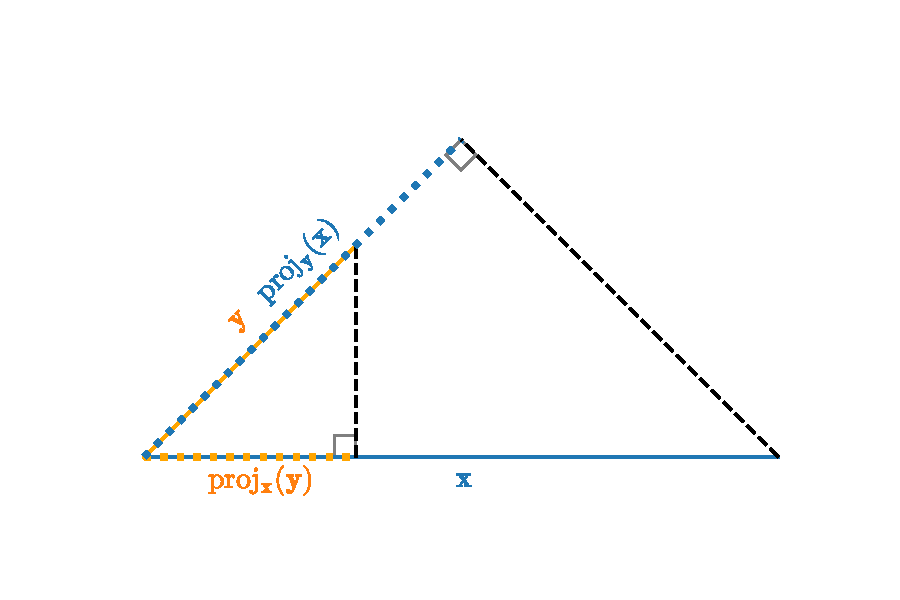
\includegraphics[width=0.8\linewidth, trim={2.1cm 17mm 2cm 20mm}, clip]{KandFigur4.pdf}
	\caption{\label{fig:proj}Två vektorer, $\bfx$ i blått och $\bfy$ i orange, samt projektionen av $\bfx$ på $\bfy$ streckat i blått och projektionen av $\bfy$ på $\bfx$ streckat i orange. Streckat i svart finns de ortogonala vektorerna.}
\end{figure}

Låt $\bfx,~\bfy\in\hil$ vara två vektorer olika $\mathbf{0}$. Välj $\lambda\in\mathbb{R}$ så att vektorn $\left(\bfx-\lambda\bfy \right)$ är ortogonal till $\bfy$ det vill säga
\begin{equation*}
	\inner{\bfx-\lambda\bfy}{\bfy}_\hil=\inner{\bfx}{\bfy}_\hil-\lambda\inner{\bfy}{\bfy}_\hil=0.
\end{equation*}
När man löser för $\lambda$ får man då
\begin{equation*}
	\lambda=\frac{\inner{\bfx}{\bfy}_\hil}{\inner{\bfy}{\bfy}_\hil}.
\end{equation*}
Talet $\lambda$ är alltså hur långt längs med $\bfy$ man ska ta sig för att vektorn $\left(\bfx-\lambda\bfy\right)$ ska vara ortogonal till $\bfy$.
Man kallar talet $\lambda$ för vektorn $\bfx$:s komponent i $\bfy$:s riktning.
Vektorn $\lambda\bfy$ kallar man projektionen av $\bfx$ på $\bfy$.
Man får alltså definitionen:
\begin{defi}[Enligt \cite{Lang}]
	För två vektorer $\bfx,~\bfy\in\mathcal{H}$ olika $\mathbf{0}$. Definiera \emph{komponenten} av $\bfx$ i $\bfy$:s riktning, $\operatorname{comp}_\bfy\left(\bfx\right)$, som talet  
	\begin{equation*}
		\operatorname{comp}_\bfy\left(\bfx\right)=\frac{\inner{\bfx}{\bfy}_\hil}{\inner{\bfy}{\bfy}_\hil}
	\end{equation*}
	och \emph{projektionen} av $\bfx$ på $\bfy$, $\operatorname{proj}_\bfy\left(\bfx\right)$, som
	\begin{equation*}
		\operatorname{proj}_\bfy\left(\bfx\right)=\operatorname{comp}_\bfy\left(\bfx\right)\bfy=\frac{\inner{\bfx}{\bfy}_\hil}{\inner{\bfy}{\bfy}_\hil}\bfy.
	\end{equation*}
\end{defi}
\begin{rem}
	Ifall vektorn $\bfy$ är normaliserad det vill säga $\left\|\bfy\right\|_\hil=1$ så är $\operatorname{comp}_\bfy\!\left(\bfx\right)=\left\|\operatorname{proj}_\bfy\!\left(\bfx\right)\right\|_\hil$ ifall $\operatorname{comp}_\bfy\!\left(\bfx\right)\geq0$ och $\operatorname{comp}_\bfy\!\left(\bfx\right)=-\!\left\|\operatorname{proj}_\bfy\!\left(\bfx\right)\right\|_\hil$ ifall $\operatorname{comp}_\bfy\left(\bfx\right)\leq0$.
	Märk även att för $\bfx=\mathbf{0}$ så går det att definiera komponenter och projektioner på samma sätt men de är inte speciellt intressanta, $\operatorname{comp}_\bfy\left(\bfx\right)=0$ och $\operatorname{proj}_\bfy\left(\bfx\right)=\operatorname{comp}_\bfy\left(\bfx\right)\bfy=\mathbf{0}$.
	Vektorn $\bfy$ måste däremot vara olika $\mathbf{0}$ för att undvika division med 0.
	Ifall vektorerna $\bfx,~\bfy$ är parallella det vill säga $\bfy=\lambda\bfx$ gäller $\operatorname{comp}_\bfx\left(\bfy\right) = \operatorname{comp}_\bfx\left(\lambda\bfx\right) = \frac{\inner{\lambda \bfx}{\bfx}_\hil}{\inner{\bfx}{\bfx}_\hil} = \frac{\lambda \inner{\bfx}{\bfx}_\hil}{\inner{\bfx}{\bfx}_\hil}=\lambda$ och $\operatorname{proj}_\bfx\left(\bfy\right)=\lambda\bfx=\bfy$. För $\operatorname{proj}_\bfy\left(\bfx\right)$ gäller $\operatorname{proj}_\bfy\left(\bfx\right) = \operatorname{proj}_\bfy\left(\frac{1}{\lambda}\bfy\right)=\operatorname{comp}_\bfy\left(\bfx\right)\bfy = \frac{\inner{\frac{1}{\lambda}\bfy}{\bfy}_\hil}{\inner{\bfy}{\bfy}_\hil}\bfy= \frac{1}{\lambda}\bfy=\bfx$.
\end{rem}

Märk hur dimensionen på vektorrummet $X$ inte nämns i definitionen för inreprodukten och därför kan Hilbertrum även vara oändligtdimensionella. Många av de bekanta egenskaperna för ändligtdimensionella inreproduktrum gäller även för oändligtdimensionella inreproduktrum, ett exempel är Hilbertrummet $\mathcal{L}^2$ med inreprodukten $\inner{f}{g}_{\mathcal{L}^2}$ som behandlades tidigare. För $\mathcal{L}^2$ gäller fortfarande att två funktioner $f$ och $g$ är ortogonala om
\begin{equation*}
	\inner{f}{g}_{\mathcal{L}^2}=\int_{a}^{b}f(x)g(x) \, dx=0,
\end{equation*}
även om det kan vara svårt att visualisera för oändligtdimensionella rum.

För att hjälpa till med visualiseringen av oändligtdimensionella rum finns ett till verktyg som ger en parallell till de ändligtdimensionella vektorrummens koordinatsystem och basvektorer. För att undersöka saken är det naturligt att leta efter något som kunde agera som motsvarighet till basvektorerna. Ett sådant koncept finns om det existerar en \emph{ortonormal följd} av vektorer, $\mathbf{e}_i$, $i=1,~2,~3,~\dots$, det vill säga en följd vektorer sådana att $\left\|\mathbf{e}_i\right\|_\hil=1$, $i=1,~2,~3,~\dots$, och $\inner{\mathbf{e}_i}{\mathbf{e}_j}_\hil=0$ om $i\neq j$.

\begin{ex}
I $\mathcal{L}^2$, $x\in\left[-\pi,\pi\right]$ är följande en ortonormal följd \cite{Young}:
\begin{equation*}
	\mathbf{e}_1=\frac{1}{\sqrt{2\pi}},\quad\mathbf{e}_2=\frac{1}{\sqrt{\pi}}\cos\left(x\right),\quad\mathbf{e}_3=\frac{1}{\sqrt{\pi}}\sin\left(x\right),\quad\mathbf{e}_2=\frac{1}{\sqrt{\pi}}\cos\left(2x\right),~\dots
\end{equation*}
\end{ex}


\begin{defi}[Enligt \cite{Young}]
	En ortonormal följd basvektorer $\mathbf{e}_i$ i ett Hilbertrum $\hil$ är \emph{fullständig} (inte samma som definition \ref{def:Cfull}) ifall nollvektorn $\mathbf{0}$ är den enda vektorn i $\hil$ ortogonal till varje basvektor $\mathbf{e}_i$. Vidare är ett Hilbertrum \emph{separabelt} ifall det existerar en fullständig ortonormal följd basvektorer $\mathbf{e}_i\in\hil$.
\end{defi}

Det visar sig att inte alla Hilbertrum har en motsvarighet till basvektorer men ifall Hilbertrummet är separabelt så existerar det en ortonormal följd vektorer sådan att för varje vektor $\mathbf{x}\in \mathcal{H}$  gäller \cite{Young}:
\begin{equation*}
\mathbf{x}=\sum_{i=1}^{\infty}\left\langle \mathbf{x}, \mathbf{e}_i \right\rangle_\hil \mathbf{e}_i,
\end{equation*}
där vektorerna $\mathbf{e}_i$ agerar bas och koefficienten $\left\langle \mathbf{x}, \mathbf{e}_i \right\rangle_\hil$ kallas den $i$:te Fourierkoefficienten med avseende på basen $\mathbf{e}_i,$ $i=1,~2,~3,~\dots$.
Märk att man projicerar $\bfx$ på varje basvektor $\mathbf{e}_i$ och summerar de resulterande projektionerna.
Antalet basvektorer $\mathbf{e}_i$ bestämmer i princip dimensionen på Hilbertrummet.

%\begin{ex}
%I $\mathcal{L}^2$, $x\in\left[-\pi,\pi\right]$ är följande en ortonormal följd basvektorer \cite{Young}:
%\begin{equation*}
%	\mathbf{e}_1=\frac{1}{\sqrt{2\pi}},\quad\mathbf{e}_2=\frac{1}{\sqrt{\pi}}\cos\left(x\right),\quad\mathbf{e}_3=\frac{1}{\sqrt{\pi}}\sin\left(x\right),\quad\mathbf{e}_2=\frac{1}{\sqrt{\pi}}\cos\left(2x\right),~\dots
%\end{equation*}
%\end{ex}

%\begin{defi}[Enligt \cite{Young}]
%	En ortonormal följd basvektorer $\mathbf{e}_i$ i ett Hilbertrum $\hil$ är \emph{fullständig} (inte samma som definition \ref{def:Cfull}) ifall nollvektorn $\mathbf{0}$ är den enda vektorn i $\hil$ ortogonal till varje basvektor $\mathbf{e}_i$. Vidare är ett Hilbertrum \emph{separabelt} ifall det existerar en fullständig ortonormal följd basvektorer $\mathbf{e}_i\in\hil$.
%\end{defi}

%I fortsättningen behandlas bara separabla Hilbertrum, så att varje vektor $\mathbf{x}$ kan skrivas som en linjär kombination av basvektorerna.

\chapter{Stödvektormaskiner (SVM)}

\section{Klassificering med hjälp av separerande hyperplan}

Inom statistiken och maskininlärningen finns många olika metoder för att försöka lösa \emph{klassificeringsproblem}, till exempel med hjälp av regressionsmodeller eller klusteranalys.

\begin{defi}
	Ett \textit{klassificeringsproblem} är ett problem var man utgående från en mängd observationspar (\textit{träningsdata}) $\left(\mathbf{x}_i, y_i\right)$, med $\mathbf{x}_i\in\mathbb{R}^p$ och $y_i\in\{-1, 1\}$ för $i=1,~\dots,~N$, försöker hitta en regel $g: \mathbb{R}^p \longmapsto \{-1, 1\}$ sådan att $g\left(\mathbf{x}_i\right)=y_i$ för så många observationspar $\left(\mathbf{x}_i, y_i\right)$ som möjligt.
\end{defi}

 I detta kapitel behandlas en metod för att lösa klassificeringsproblem som använder ett \emph{hyperplan}, det vill säga ett affint underrum med dimensionen $p-1$, för att klassificera \textit{observationerna} $\mathbf{x}_i$ i \textit{klasserna} $y_i\in\{-1, 1\}$.

\begin{defi}
	Ett \textit{hyperplan} i ett inreproduktrum $\mathcal{H}$ är ett affint underrum av $\mathcal{H}$ definierat som mängden $\{\mathbf{x}: \inner{\bfx}{\bfbeta}_\mathcal{H} + \beta_0=0\}$, med $\mathbf{x},~\bfbeta\in X$ och $\beta_0\in\mathbb{R}$.
%	\\Klassificeringsregeln $g$ för separerande hyperplan blir
%	\begin{equation*}
%	g\left(\mathbf{x}_i\right)=  
%	\begin{cases}
%	~~ 1 &\text{ om } \inner{\bfx_i}{\bfbeta}_\hil + \beta_0 \geq 0,\\
%	-1 &\text{ om } \inner{\bfx_i}{\bfbeta}_\hil + \beta_0 < 0,
%	\end{cases}\qquad\text{där }\bfx_i\text{ är en observation.}
%	\end{equation*}
\end{defi}

\begin{ex}
	I figur \ref{fig:separatinghyperplane} illustreras två separerande hyperplan i $\mathbb{R}^2$. I $\mathbb{R}^2$ blir hyperplanet en linje, med andra ord ett affint underrum med dimensionen $2-1=1$.
	Allmänt gäller att i ett rum med dimensionen $p$ blir hyperplanet ett affint underrum med dimensionen $p-1$.
	Märk att ifall punkten\footnote{I resten av avhandlingen kommer begreppen \emph{punkter} och \emph{vektorer} att användas om vartannat. Egentligen är alla punkter också vektorer i samma vektorrum som resten av vektorerna men i litteraturen används ofta punkter eftersom det är hur man intuitivt brukar tänka på uppmätta observationer. Vektorer brukar användas om man vill poängtera att riktningen är viktigt.} $\bfx = 0$ tillhör hyperplanet så är hyperplanet ett underrum.
\end{ex}

För nästa sats behövs några konventioner för ett hyperplan $L=\sephyp$ i relation till en punkt
$\bfy$ i $\hil$:
\begin{itemize}
	\item Man säger att punkten $\bfy$ ligger över hyperplanet $L$ om $f\left(\bfy\right)>0$ och under om $f\left(\bfy\right)<0$.
%	\item På samma sätt säger man att $\bfbeta$ pekar mot punkten $\bfy$ om $f\left(\bfy\right)>0$.
	\item Det signerade avståndet från punkten $\bfy$ till hyperplanet $L$, $\operatorname{d}^\pm\!\left(\bfy, L\right)$, definieras som $\inf_{\bfx\in L} \left\|\bfy-\bfx\right\|_\hil$ om $f\left(\bfy\right)\geq0$ och $-\left(\inf_{\bfx\in L} \left\|\bfy-\bfx\right\|_\hil\right)$ om $f\left(\bfy\right)\leq0$.
	Med andra ord är $\operatorname{d}^\pm\left(\bfy,L\right)$ det kortaste avståndet (med avseende på den inducerade normen i $\hil$) från punkten $\bfy$ till alla punkter $\bfx\in L$ om $\bfy$ ligger över $L$ och minus det kortaste avståndet från $\bfy$ till $L$ om $\bfy$ ligger under $L$.
\end{itemize}

\begin{thm}[Enligt \cite{ESL}]\label{thm:hyperplan}
	Ett hyperplan i ett inreproduktrum $\hil$ definierat som den affina mängden $L=\sephyp$ har följande egenskaper:
	\begin{enumerate}
		\item Vektorn $\bfbeta$ är ortogonal till alla vektorer i $L$ (det vill säga alla vektorer sådana att ändpunkterna ligger i $L$) och kan \emph{ortonormeras} (göras ortonormal) genom
		\begin{equation*}
			\widehat{\bfbeta} = \frac{\bfbeta}{\left\|\bfbeta\right\|_\hil}.
		\end{equation*}
		\item $\inner{\bfx_0}{\bfbeta}_\hil = -\beta_0$ för alla $\mathbf{x}_0$ i $L$.
		\item
		För det signerade avståndet från en punkt $\mathbf{y}$ till hyperplanet $L$ gäller att
		\begin{align*}
			\operatorname{d}^\pm \left(\mathbf{y}, L\right) &=\inner{\mathbf{y}-\mathbf{x}_0}{\widehat{\bfbeta}}_\hil\\
			&=\frac{1}{\left\|\bfbeta\right\|_\hil}\left(\inner{\mathbf{y}}{\bfbeta}_\hil+\beta_0\right)\\
\intertext{där $\bfx_0$ är en godtycklig punkt i hyperplanet $L$. Om $\hil$ är lika med $\mathbb{R}^p$ med den vanliga inreprodukten fås dessutom}
			\operatorname{d}^\pm \left(\mathbf{y}, L\right)			&=\frac{1}{\left\|f^\prime\left(\mathbf{y}\right)\right\|_p}f\left(\mathbf{y}\right).
		\end{align*}
	\end{enumerate}
\end{thm}
\begin{proof} (Inte från \cite{ESL}.)
	\leavevmode
\begin{enumerate}
	\item Låt $\mathbf{x}_1$ och $\mathbf{x}_2$ vara två godtyckliga punkter i $L$. Då gäller att $f\left(\mathbf{x}_1\right)=f\left(\mathbf{x}_2\right)=0$ och
	\begin{align*}
		0 &= f\left(\mathbf{x}_1\right)-f\left(\mathbf{x}_2\right)\\
		&= \inner{\bfx_1}{\bfbeta}_\hil + \beta_0 - \inner{\bfx_2}{\bfbeta}_\hil - \beta_0\\
		&= \inner{\mathbf{x}_1-\mathbf{x}_2}{\bfbeta}_\hil
	\end{align*}
	med andra ord är $\bfbeta$ ortogonal till vektorn $\left(\mathbf{x}_1-\mathbf{x}_2\right)$, det vill säga vektorn från en punkt i $L$ till en annan punkt i $L$.
	Dessutom gäller för $\widehat{\bfbeta}:=\frac{\bfbeta}{\left\|\bfbeta
	\right\|_p}$ att $\left\|\widehat{\bfbeta}\right\|_\hil=1$ så $\widehat{\bfbeta}$ är ortonormal till alla vektorer i $L$. \hfill\qedsymbol

	\item \label{eq:egenskap2}Låt $\mathbf{x}_0$ vara en punkt i $L$. Då gäller att $f\left(\mathbf{x}_0\right)=\inner{\bfx_0}{\bfbeta}_\hil + \beta_0 = 0$ alltså är $\inner{\bfx_0}{\bfbeta}_\hil = - \beta_0$.\hfill \qedsymbol
	
	\item Låt $\mathbf{x}_0$ vara en punkt i hyperplanet $L$, då är avståndet från punkten $\bfx_0$ till punkten $\bfy$ minimerat om vektorn $\left(\bfy-\bfx_0\right)$ är ortogonal till hyperplanet -- i $\mathbb{R}^2$ är detta principen att det kortaste avståndet från en linje till en punkt är avståndet mätt längs med en linje vinkelrät mot den ursprungliga linjen.
	Eftersom $\widehat{\bfbeta}$ är ortonormal till varje punkt i $L$ så blir det kortaste avståndet från $\bfy$ till $L$ längden av projektionen av vektorn från $\bfx_0$ till $\bfy$ på $\widehat{\bfbeta}$ det vill säga $\operatorname{d}^\pm \left(\mathbf{y}, L\right)=\operatorname{comp_{\widehat{\bfbeta}}} \left( \bfy - \mathbf{x}_0 \right)$.
	Vidare fås då
	\begin{align*}
		\operatorname{d^\pm} \left( \bfy, L \right) &= \operatorname{comp_{\widehat{\bfbeta}}} \left( \bfy - \mathbf{x}_0 \right)
		=\underline{\underline{ \inner{\bfy - \mathbf{x}_0}{\widehat{\bfbeta}}_\hil}}\\
		&= \frac{1}{\left\|\bfbeta
\right\|_\hil}\left(\inner{\bfy}{\bfbeta}_\hil - \inner{\bfx_0}{\bfbeta}_\hil\right)=\underline{\underline{\frac{1}{\left\|\bfbeta
\right\|_\hil}\left(\inner{\bfy}{\bfbeta}_\hil + \beta_0\right)}}
	\end{align*}
	där det sista steget följer från egenskap \ref{eq:egenskap2} då $\mathbf{x}_0$ är en punkt i $L$.
	Om $\hil$ är lika med $\mathbb{R}^p$ och inreprodukten ges av $\inner{\bfx}{\bfy}_p=\bfx^\intercal\bfy$ kan man noterar att $f\left(\bfy\right)=\inner{\bfy}{\bfbeta}_p+\beta_0$ och $f^\prime\left(\bfy\right)=\bfbeta$, då fås även att
	\begin{equation*}
		\operatorname{d^\pm} \left( \bfy, L \right)=\frac{1}{\left\|\bfbeta
\right\|_p}\left(\inner{\bfy}{\bfbeta}_p + \beta_0\right)=\frac{1}{\left\|f^\prime\left(\bfy\right)
\right\|_p}f\left(\bfy\right).
	\end{equation*}
	\qedhere
\end{enumerate}
\end{proof}

\begin{rem}
	Definitionen $L=\{ \mathbf{x} : f\left(\mathbf{x}\right)=\inner{\bfx}{\bfbeta}_\hil + \beta_0=0\}$ för hyperplanet $L$ är inte entydig.
\end{rem}
\begin{reas}
	Betrakta hyperplanen $L_1 = \sephyp$ och $L_2 = \left\{\mathbf{x}: g\left(\mathbf{x}\right)=\inner{\bfx}{-\bfbeta}_\hil + \left(-\beta_0\right) = 0\right\}$. Eftersom $g\left(\mathbf{x}\right) = -f\left(\mathbf{x}\right)$ så gäller att om $\mathbf{x}_0$ tillhör $L_1$ så tillhör $\mathbf{x}_0$ även $L_2$.
	Betrakta vidare hyperplanet $L_3= \left\{\mathbf{x}: h\left(\mathbf{x}\right)=\frac{\inner{\bfx}{\bfbeta}_\hil}{\left\|\bfbeta
\right\|_\hil} + \frac{\beta_0}{\left\|\bfbeta
\right\|_\hil}=0\right\}$. Om punkten $\mathbf{x}_0$ tillhör $L_1$ så tillhör punkten $\mathbf{x}_0$ även $L_3$ eftersom $h\left(\mathbf{x}\right) = \frac{f\left(\mathbf{x}\right)}{\left\|\bfbeta
\right\|_\hil}=0$. Notera även att $\frac{1}{\left\|\bfbeta
\right\|_\hil}$ kunde ha varit vilket reellt tal som helst.
\end{reas}

\begin{rem}
	För att få entydiga hyperplan för klassificering kan man lägga till villkor. Om man kräver att $\left\|\bfbeta\right\|_\hil=1$ och $y_i\left(\inner{\bfx_i}{\bfbeta}_\hil + \beta_0\right)\geq0$ för alla $i=1,~\dots,~N$, där $\left(\bfx_i, y_i\right)$ är observationsparen i klassificeringsproblemet, så får man en entydig definition av hyperplanet där observationerna $\bfx_i$ i klassen $y_i=1$ ligger över hyperplanet medan observationerna $\bfx_i$ i klassen $y_i=-1$ ligger under.
	Dessutom anger $\beta_0$ det signerade avståndet från origo till hyperplanet (i relation till riktningen på $\bfbeta$).
\end{rem}
\begin{reas}
	De extra villkoren gör att man inte längre kan göra manipulationerna som påvisade icke-entydigheten. Om man sätter $\mathbf{x}=\mathbf{0}$ så får man med hjälp av sats \ref{thm:hyperplan} att det signerade avståndet från origo till hyperplanet är lika med
	\begin{equation*}
	\frac{1}{\left\|\bfbeta
\right\|_p}\left(\inner{\bfx}{\bfbeta}_\hil+\beta_0\right)=\frac{1}{\left\|\bfbeta
\right\|_p}\left(\inner{\mathbf{0}}{\bfbeta}_\hil+\beta_0\right)=\beta_0.
	\end{equation*}
\end{reas}

\begin{figure}[h]
\centering
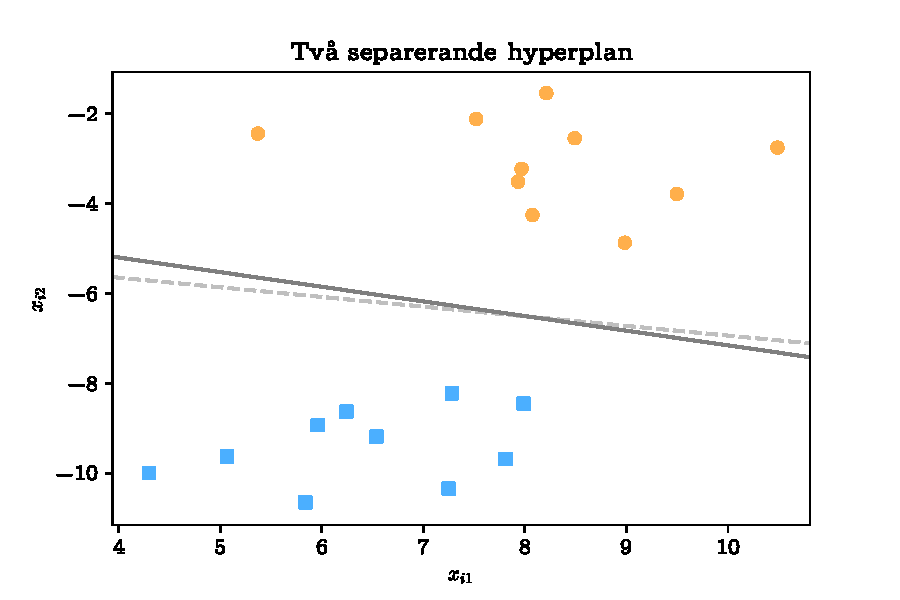
\includegraphics[width=0.8\linewidth, trim={0.5cm 2mm 0.5cm 6mm}, clip]{KandFigur1.pdf}
\caption{\label{fig:separatinghyperplane}20 datapunkter med två separerande hyperplan (linje) där klassen $y_i=1$ framställs som blå fyrkanter och klassen $y_i=-1$ som orangea cirklar.}
\end{figure}

\begin{defi}
	Ett klassificeringsproblem eller en mängd observationspar $\left(\mathbf{x}_i, y_i\right)$ är \textit{linjärt separabelt} om det existerar ett hyperplan $L=\sephyp$ sådant att punkten $\bfx_i$ ligger över hyperplanet om $y_i=1$ och under om $y_i=-1$. Ett sådant hyperplan kallas ett \emph{separerande hyperplan}.
\end{defi}
\begin{rem}
	Genom att byta tecken på $\bfbeta$ och $\beta_0$ kan man se att ifall det existerar ett hyperplan $\sephyp$ sådant att punkten $\bfx_i$ ligger under hyperplanet om $y_i=1$ och över om $y_i=-1$ så finns även ett sådant att punkten $\bfx_i$ ligger över hyperplanet om $y_i=1$ och under om $y_i=-1$.
	Konventionen är att man väljer det hyperplan som passar ovanstående definition.
\end{rem}
\begin{thm}[Enligt \cite{Boyd}]\label{thm:sephyppositive}
	För ett separerande hyperplan $L=\sephyp$ gäller att 
	\begin{equation*}
		y_i\left(\inner{\bfx_i}{\bfbeta}_\hil + \beta_0\right) > 0
	\end{equation*}
	för alla $i = 1,~\dots,~N$.
\end{thm}
\begin{proof}
	Ifall ett klassificeringsproblem är linjärt separabelt så ligger alla observationer $y_i$ på rätt sida om det separerande hyperplanet. Detta betyder att ifall $y_i=1$ så är $\inner{\bfx_i}{\bfbeta}_\hil + \beta_0 > 0$ och om $y_i=-1$ så är $\inner{\bfx_i}{\bfbeta}_\hil + \beta_0 < 0$.
	Då fås $y_i\left(\inner{\bfx_i}{\bfbeta}_\hil + \beta_0\right) > 0$. Ifall $\inner{\bfx_i}{\bfbeta}_\hil + \beta_0 = 0$ är problemet inte linjärt separabelt.
\end{proof}

Klassificeringsregeln $g$ för separerande hyperplan blir
\begin{equation*}
g\left(\mathbf{x}_i\right)=  
\begin{cases}
~~ 1 &\text{ om } \inner{\bfx_i}{\bfbeta}_\hil + \beta_0 > 0,\\
-1 &\text{ om } \inner{\bfx_i}{\bfbeta}_\hil + \beta_0 < 0,
\end{cases}\qquad\text{där }\bfx_i\text{ är en observation.}
\end{equation*}

\begin{ex}\label{exempel:mångahyperplan}%TODO	Komma? Semikolon?
	Låt observationsparen vara $\left(\left[2,~2\right]^\intercal\!,~1\right),~\left(\left[1,~2\right]^\intercal\!,-1\right)$, inreproduktrummet i fråga är då $\mathbb{R}^2$ och inreprodukten $\inner{\bfx}{\mathbf{y}}_2:=\bfx^\intercal\mathbf{y}$. Då är $$L_1=\{\mathbf{x}\in\mathbb{R}^2: \mathbf{x}^\intercal\begin{bmatrix}
	1\\
	0
	\end{bmatrix} - 1,5=0\}$$ och $$L_2=\{\mathbf{x}\in\mathbb{R}^2: \mathbf{x}^\intercal\begin{bmatrix}
	\sqrt{2}\\
	\sqrt{2}
	\end{bmatrix} - 3,5\sqrt{2}=0\}$$ två separerande hyperplan (linjer i detta fall).
\end{ex}
\begin{proof}
	För $L_1$: $$y_1\left(\mathbf{x}_1^\intercal\begin{bmatrix}
	1\\
	0\end{bmatrix}-1,5\right)=\left[2,~2\right]\begin{bmatrix}
	1\\
	0\end{bmatrix}-1,5=0,5>0$$ och $$y_2\left(\mathbf{x}_2^\intercal\begin{bmatrix}
	1\\
	0\end{bmatrix}-1,5\right)=-1\left(\left[1,~2\right]\begin{bmatrix}
	1\\
	0\end{bmatrix}-1,5\right)=\left(-1\right)\left(-0,5\right)=0,5>0.$$
	Och för $L_2$: $$y_1\left(\mathbf{x}_1^\intercal\begin{bmatrix}
	\sqrt{2}\\
	\sqrt{2}\end{bmatrix}-3,5\sqrt{2}\right)=\left[2,~2\right]\begin{bmatrix}
	\sqrt{2}\\
	\sqrt{2}\end{bmatrix}-3,5\sqrt{2}=0,5\sqrt{2}>0$$ och
	\begin{align*}
	y_2\left(\mathbf{x}_2^\intercal\begin{bmatrix}
	\sqrt{2}\\
	\sqrt{2}\end{bmatrix}-3,5\sqrt{2}\right)&=-1\left(\left[1,~2\right]\begin{bmatrix}
	\sqrt{2}\\
	\sqrt{2}\end{bmatrix}-3,5\sqrt{2}\right)\\
	&=\left(-1\right)\left(-0,5\sqrt{2}\right)=0,5\sqrt{2}>0
	\end{align*}
\end{proof}

\begin{rem}
	Hyperplan i $\mathbb{R}^p$ kan konstrueras enkelt genom att man väljer $p$ stycken punkter $\mathbf{x}_i$ som man vill att hyperplanet ska gå igenom, sedan löser man ekvationssystemet $X\bfbeta=-\beta_0\mathbf{1}$, i vilket $X$ är en matris där raderna består av punkterna $\mathbf{x}_i^\intercal$, $i=1,\dots, p$, och $\beta_0\mathbf{1}$ är en vektor med värdet $\beta_0$ i alla rader.
	Med andra ord löser man ekvationssystemet
	\begin{equation*}
		\begin{bmatrix}
		\bfx_{1,1}	& \bfx_{1,2}	& \cdots	& \bfx_{1,p-1}	& \bfx_{1,p}\\
		\bfx_{2,1}	& \bfx_{2,2}	&  			& 				& \bfx_{2,p}\\
		\vdots		&				& \ddots	&				& \vdots\\
		\bfx_{p-1,1}& 				&  			& \bfx_{p-1,p-1}	&\bfx_{p-1,p}\\
		\bfx_{p,1}	& \bfx_{p,2}	& \cdots	& \bfx_{p,p-1}	& \bfx_{p,p}\\
		\end{bmatrix}
		\begin{bmatrix}
		\bfbeta_1\\ \bfbeta_2\\\vdots\\\bfbeta_{p-1}\\\bfbeta_{p}
		\end{bmatrix}=
		\begin{bmatrix}
		-\beta_0\\-\beta_0\\\vdots\\-\beta_0\\-\beta_0
		\end{bmatrix},
	\end{equation*}
	ekvationssystemet kan aldrig vara överbestämt men nog underbestämt ifall punkterna inte är linjärt oberoende.
\end{rem}

Som syns i exempel \ref{exempel:mångahyperplan} finns det ofta många separerande hyperplan om ett klassificeringsproblem är linjärt separabelt och frågan är då vilket separerande hyperplan man borde välja.

\section{Optimala separerande hyperplan}
Metoder för att modellera data inom statistik och maskininlärning kan ofta visas vara ekvivalenta med något optimeringsproblem, till exempel maximum likelihood-metoden för linjär regression, som är ekvivalent med minsta-kvadratmetoden \cite{MLEOLS}.
Optimeringsproblemen kan ofta ändras genom att man lägger till eller tar bort termer i objektfunktionen eller ändrar på kraven och på så sätt får en ny metod (för att modellera data) med andra egenskaper.

För metoden med optimalt separerande hyperplan är tanken att om man hittar ett hyperplan sådant att:
\begin{itemize}
	\item alla observationer klassificeras rätt och,
	\item hyperplanet samtidigt maximerar det kortaste avståndet från hyperplanet till det närmsta observationsparet,
\end{itemize}
så borde hyperplanet även fungera bra för att separera och klassificera nya observationer \cite{VapnikLerner1963}.
Matematiskt kan man uttrycka problemet som följande optimeringsproblem
\begin{equation}\label{opt:optimalmargin1}
\begin{aligned}
	 \operatornamewithlimits{max}_{\widehat{\bfbeta}, \widehat{\beta}_0, \left\|\widehat{\bfbeta}\right\|_p=1}& & &C\\
	 \text{så att}& & &y_i\left(\inner{\bfx_i}{\widehat{\bfbeta}}_p+\widehat{\beta}_0\right)\geq C,\quad i=1,~\dots,~N
\end{aligned}
\end{equation}
där $C$ kallas \emph{marginalen} och betecknar avståndet från hyperplanet till de närmaste observationerna. Här betecknar $\left(\bfx_i, y_i\right)$ observationsparen i träningsdatat där $\bfx_i\in\mathbb{R}^p$ och $y_i\in\left\{-1, 1 \right\}$ för $i=1,~\dots,~N$, detta gäller även för resten av kapitlet om inte annat anges.
\begin{rem}
	Ifall alla punkter är rätt klassificerade ger sats \ref{thm:hyperplan} och \ref{thm:sephyppositive} att $y_i\left(\inner{\bfx_i}{\widehat{\bfbeta}}_p+\widehat{\beta}_0\right)$ är det absoluta avståndet mellan hyperplanet och punkten $\mathbf{x}_i$.
\end{rem}

Förhoppningen är att om man väljer det separerande hyperplan som befinner sig så långt som möjligt från båda klasserna får man ett hyperplan som även generaliserar väl till ny data. Dessutom är detta även ett unikt sätt att välja ett separerande hyperplan det vill säga optimeringsproblemet är konvext \cite{ESL}. %TODO definiera konvext

För att visa att optimeringsproblemet (\ref{opt:optimalmargin1}) är \textit{konvext} måste det skrivas om. Idén är att man låter inversen av längden på vektorn $\bfbeta$ beskriva avståndet till närmast punkt, då skapas en direktare länk mellan kraven och objektfunktionen i optimeringsproblemet.

Först måste alltså kravet $\left\|\widehat{\bfbeta}
\right\|_p=1$ bytas ut. Detta görs genom att man byter ut kraven
\begin{equation*}
y_i\left(\inner{\bfx_i}{\widehat{\bfbeta}}_p+\widehat{\beta}_0\right)\geq C,\quad i=1,~\dots,~N
\end{equation*}
mot kraven
\begin{equation*}
y_i\left(\inner{\bfx_i}{\frac{\bfbeta}{\left\|\bfbeta
\right\|_p}}_p+\frac{\beta_0}{\left\|\bfbeta
\right\|_p}\right) = 
\frac{1}{\left\|\bfbeta
\right\|_p}y_i\left(\inner{\bfx_i}{\bfbeta}_p+\beta_0\right)
 \geq C,\quad i=1,~\dots,~N
\end{equation*}
eller ekvivalent
\begin{equation*}
y_i\left(\inner{\bfx_i}{\bfbeta}_p+\beta_0\right)\geq C\left\|\bfbeta
\right\|_p,\quad i=1,~\dots,~N,
\end{equation*}
där man valt en av de andra representationerna för samma hyperplan genom att skala om $\widehat{\bfbeta}$ och $\widehat{\beta}_0$. Vidare kan $C$ elimineras genom att man väljer $C=\frac{1}{\left\|\bfbeta
\right\|_p}$, då fås
\begin{equation*}
y_i\left(\inner{\bfx_i}{\bfbeta}_p+\beta_0\right)\geq 1,\quad i=1,~\dots,~N
\end{equation*}
och eftersom $C=\frac{1}{\left\|\bfbeta
\right\|_p}$ är en avtagande funktion med avseende på $\left\|\bfbeta
\right\|_p$ är maximering av $C$ ekvivalent med minimering av $\left\|\bfbeta
\right\|_p$ och motsvarande optimeringsproblem blir
\begin{equation*}%\label{opt:optimalmargin2}
\begin{aligned}
\operatornamewithlimits{min}_{\bfbeta, \beta_0} & & &\left\|\bfbeta
\right\|_p\\
\text{så att} & & &y_i\left(\inner{\bfx_i}{\bfbeta}_p+\beta_0\right)\geq 1,\quad i=1,~\dots,~N.
\end{aligned}
\end{equation*}
Därefter görs ännu en konvexitetsbevarande kvadratisk transformering av objektfunktionen\footnote{Inom statistik- och maskinilärningslitteraturen kallas objektfunktionen ibland även för \textit{kostfunktionen}.} $\left\|\bfbeta\right\|_p$, det vill säga man noterar att om $\bfbeta^*$ är sådan att $\operatornamewithlimits{min}_{\bfbeta, \beta_0} \left\|\bfbeta\right\|_p=\left\|\bfbeta^*\right\|_p$ gäller så gäller även $\operatornamewithlimits{min}_{\bfbeta, \beta_0} \frac{1}{2}\left\|\bfbeta\right\|_p^2=\frac{1}{2}\left\|\bfbeta^*\right\|_p^2$ för samma $\bfbeta^*$.
Detta brukar betecknas med funktionen $\operatornamewithlimits{argmin}_{\bfbeta,\beta_0} \left(f\left(\bfy\right)\right)$ som ger som resultat det $\bfy^*$ som minimerar funktionen $f\left(\bfy\right)$.

%\begin{equation*}%TODO Definiera argmin
%\operatornamewithlimits{argmin}_{\bfbeta,\beta_0} \left\|\bfbeta
%\right\|_p=\operatornamewithlimits{argmin}_{\bfbeta,\beta_0} \frac{1}{2}\left\|\bfbeta
%\right\|_p^2.
%\end{equation*}
En orsak till att göra den kvadratiska transformeringen är att man på så sätt kan garantera att objektfunktionen är deriverbar:
\begin{ex}
	Låt $x\in\mathbb{R}$, $f\left(x\right):=|x-x_0|$ och $g\left(x\right):=\left(f\left(x\right)\right)^2$. Då är $f\left(x\right)$ inte deriverbar i punkten $x_0$ medan $D_x\left(g\left(x\right)\right)=D_x\left(\left(x-x_0\right)^2\right)=D_x\left(x^2-2xx_0+x_0^2\right)=2x-2x_0=2\left(x-x_0\right)$ och $D_x\left(g\left(x_0\right)\right)=0$ det vill säga $\operatornamewithlimits{argmin}_x f\left(x\right) = x_0 = \operatornamewithlimits{argmin}_x g\left(x\right)$.
\end{ex}
Optimeringsproblemet \ref{opt:optimalmargin1} kan alltså skrivas på formen 
\begin{equation*}
\begin{aligned}
\operatornamewithlimits{min}_{\bfbeta, \beta_0} & & &\frac{1}{2}\left\|\bfbeta
\right\|_p^2=\frac{1}{2}\inner{\bfbeta}{\bfbeta}_p=\frac{1}{2}\bfbeta^\intercal\bfbeta=\bfbeta^\intercal\left(\frac{1}{2}I\right)\bfbeta\\
\text{så att} & & &y_i\left(\inner{\bfx_i}{\bfbeta}_p+\beta_0\right)\geq 1,\quad i=1,~\dots,~N
\end{aligned}
\end{equation*}
där $\left( \frac{1}{2}I \right)$ är en \emph{positivt semi-definit} matris, det vill säga den uppfyller kraven för att ett kvadratiskt optimeringsproblem med linjära lösbara krav ska vara konvext \cite{Boyd}.

Ovanstående resonemang är ett bevis för sats \ref{thm:primallinearproblem}.
\begin{thm}[Enligt \cite{ESL}]\label{thm:primallinearproblem}
	Låt $\widehat{\bfbeta},~\bfbeta \in \mathbb{R}^p$ och $\widehat{\beta}_0,~\beta_0 \in \mathbb{R}$. Låt dessutom observationsparen $\left(\mathbf{x}_i, y_i\right)$ vara linjärt separabla. Då är optimeringsproblemet
	\begin{equation*}
	\begin{aligned}
	\operatornamewithlimits{max}_{\widehat{\bfbeta}, \widehat{\beta}_0, \left\|\widehat{\bfbeta}
\right\|_p=1} & & &C\\
	\text{så att} & & &y_i\left(\inner{\bfx_i}{\widehat{\bfbeta}}_p+\beta_0\right)\geq C,\quad i=1,~\dots,~N
	\end{aligned}
	\end{equation*}
	konvext och man får en lösning $\left(\widehat{\bfbeta^*}, \widehat{\beta_0^*}\right)=\left(\frac{\bfbeta^*}{\left\|\bfbeta^*\right\|_p}, \frac{\beta^*_0}{\left\|\bfbeta^*\right\|_p}\right)$ genom att lösa optimeringsproblemet
	\begin{equation*}
	\begin{aligned}
	\operatornamewithlimits{min}_{\bfbeta, \beta_0} & & &\frac{1}{2}\left\|\bfbeta
\right\|_p^2\\
	\text{så att} & & &y_i\left(\inner{\bfx_i}{\bfbeta}_p+\beta_0\right)\geq 1,\quad i=1,~\dots,~N.
	\end{aligned}
	\end{equation*}
\end{thm}
%Vidare ger observationen ovan ytterligare ett ekvivalent optimeringsproblem:
%\begin{cor}\label{cor:inreproduktoptimering}
%	Optimeringsproblemen i sats \ref{thm:primallinearproblem} är ekvivalenta med optimeringsproblemet
%	\begin{equation*}
%	\begin{aligned}
%	\operatornamewithlimits{min}_{\bfbeta, \beta_0} & & &\frac{1}{2}\langle \bfbeta, \bfbeta \rangle\\
%	\text{så att} & & &y_i\left(\langle \mathbf{x}_i,\bfbeta\rangle+\beta_0\right)\geq 1,\quad i=1,~\dots,~N
%	\end{aligned}
%	\end{equation*}
%	med samma antaganden.
%\end{cor}
%\begin{proof}
%	Normen $\left\|\bfbeta
%\right\|_p=\left(\bfbeta^\intercal\bfbeta\right)^{\frac{1}{2}}$ kan uttryckas som $\langle \bfbeta, \bfbeta \rangle^{\frac{1}{2}}$ alltså är $\frac{1}{2} \left\|\bfbeta
%\right\|_p^2=\frac{1}{2}\langle \bfbeta, \bfbeta \rangle$. Resten följer från observationen.
%\end{proof}
%Framställningen i korollarium \ref{cor:inreproduktoptimering} används i många källor, bland annat i den ursprungliga framställningen för stödvektormaskinen, %TODO referens
%och är en av de mer generella framställningarna för optimeringsproblemet som stödvektormaskinen bygger på. %TODO Ha kvar det här?

\subsection{Primala och duala problem}

För att hitta alla extrempunkter till ett optimeringsproblem, det vill säga lösa ett konvext optimeringsproblem, används Lagrangemultiplikatorer \cite{Boyd}. %TODO Förklara mera utförligt? Glader vill ha förklaring för utvidgning till olikhetsvillkor men Boyd använder genast olikhetsvillkor, Tahns bok?
Den primala Lagrangefunktionen $L_P$ för optimeringsproblemet
\begin{equation*}
\begin{aligned}
\operatornamewithlimits{min}_{\bfbeta, \beta_0} & & &\frac{1}{2}\left\|\bfbeta
\right\|_p^2=\frac{1}{2}\inner{\bfbeta}{\bfbeta}_p\\
\text{så att} & & &y_i\left(\inner{\bfx_i}{\bfbeta}_p+\beta_0\right)\geq 1,\quad i=1,~\dots,~N
\end{aligned}
\end{equation*}
ges av
\begin{equation}\label{eq:primallagrange}
L_P=\frac{1}{2}\inner{\bfbeta}{\bfbeta}_p - \sum_{i=1}^{N} \lambda_i\left(y_i \left(\inner{\bfx_i}{\bfbeta}_p + \beta_0\right)-1\right)
\end{equation}
som ska minimeras med avseende på $\bfbeta$ och $\beta_0$. %TODO	Och maximeras på $\lambda$?

För att minimera $L_P$ sätts derivatorna med avseende på elementen $\left[\bfbeta\right]_j$ av $\bfbeta$ och $\beta_0$ till 0, och följande relationer erhålls:
\begin{equation}\label{eq:derivprimal}
\begin{aligned}
	D_{ \left[\bfbeta\right]_j } \left(L_P\right) &= D_{ \left[\bfbeta\right]_j } \left( \frac{1}{2} \bfbeta^\intercal \bfbeta \right) &- &D_{ \left[\bfbeta\right]_j } \left( \sum_{i=1}^{N} \left( \lambda_i y_i \left( \bfx_i^\intercal\bfbeta \right) + \lambda_i y_i \beta_0 - \lambda_i \right)\right)\\
	&= D_{ \left[\bfbeta\right]_j } \left( \frac{1}{2} \sum_{k=1}^{p} \left[\bfbeta\right]_k^2 \right)
	&- &\sum_{i=1}^{N} D_{ \left[\bfbeta\right]_j }
	\Big(  \lambda_i y_i \left( \sum_{k=1}^{p} \left[\mathbf{x}_i\right]_k \left[ \bfbeta \right]_k \right)\\
	& & &\qquad\qquad\quad+ \lambda_i y_i \beta_0-\lambda_i \Big)\\
	&= [\bfbeta]_j &- &\sum_{i=1}^{N} D_{ \left[\bfbeta\right]_j } \left( \sum_{k=1}^{p} \lambda_i y_i \left[\mathbf{x}_i\right]_k\left[\bfbeta\right]_k \right) + 0\\
	&= [\bfbeta]_j &- &\sum_{i=1}^{N}\lambda_i y_i \left[ \mathbf{x}_i \right]_j
\end{aligned}
\end{equation}
där $j=1,~\dots,~p$ och
\begin{equation*}
	D_{\beta_0}\left(L_P\right) = D_{\beta_0}\left( -\sum_{i=1}^{N} \lambda_i y_i \beta_0 \right) = -\sum_{i=1}^{N} \lambda_i y_i.
\end{equation*}
Vidare kan (\ref{eq:derivprimal}) skrivas om som derivatan med avseende på hela $\bfbeta$ eftersom $ \left[ D_{ \bfbeta }\left(L_p\right) \right]_j = D_{\left[ \bfbeta \right]_j}\left(L_p\right) $. Efter att man löser derivatorna för nollställen får man följande krav:
%tar i beaktande kraven att $ D_{ \bfbeta }\left(L_p\right) = \mathbf{0} $ och $ D_{\beta_0}\left(L_p\right)=0 $ fås följande krav:
\begin{align}\label{eq:krav1}
	\bfbeta &= \sum_{i=1}^{N} \lambda_i y_i \mathbf{x}_i\\
	0 &= \sum_{i=1}^{N} \lambda_i y_i.\label{eq:krav2}
\end{align}

Insättning av kraven (\ref{eq:krav1}) och (\ref{eq:krav2}) i $L_P$ ger följande duala problem

\begin{equation*}
\begin{aligned}
	L_D=&\frac{1}{2}\inner{\sum_{i=1}^{N}\lambda_i y_i \mathbf{x}_i}{ \sum_{j=1}^{N}\lambda_j y_j \mathbf{x}_j}_p&\\
	&- \sum_{i=1}^{N}\lambda_i \left( y_i \left(\inner{\mathbf{x}_i}{ \sum_{j=1}^{N}\lambda_j y_j \bfx_j}_p + \beta_0 \right) -1\right)&\\
	=& \frac{1}{2} \inner{\sum_{i=1}^{N} \lambda_i y_i \bfx_i}{\sum_{j=1}^{N} \lambda_j y_j \bfx_j}_p &\\
	&- \inner{\sum_{i=1}^{N}\lambda_i y_i \mathbf{x}_i}{\sum_{j=1}^{N} \lambda_j y_j \mathbf{x}_j}_p - \beta_0 \sum_{i=1}^{N} \lambda_i y_i  + \sum_{i=1}^{N} \lambda_i&\\
	=& -\frac{1}{2} \sum_{i=1}^{N} \sum_{j=1}^{N} \lambda_i \lambda_j y_i y_j \inner{\mathbf{x}_i}{\mathbf{x}_j}_p + \sum_{i=1}^{N} \lambda_i &\textstyle{\left(\sum\limits_{i=1}^{N}\lambda_iy_i = 0\right)}
\end{aligned}
\end{equation*}
som ska maximeras med avseende på $\lambda_i,~i=1,~\dots,~N,$ och kravet \begin{equation}\label{eq:krav3}
	\lambda_i\geq 0,\quad i=1,~\dots,~N.
\end{equation} Uträkningarna och kravet $\lambda_i\geq 0,~i=1,~\dots,~N,$ kan motiveras genom Karush-Kuhn-Tucker kraven \cite{Boyd} för konvexa problem, det vill säga kraven (\ref{eq:krav1}), (\ref{eq:krav2}) och (\ref{eq:krav3}) samt kravet %TODO	Skriv iallafall ut kraven för ett optimeringsproblem i allmän form
\begin{equation}\label{eq:krav4}
	\lambda_i\left( y_i\left( \inner{\bfx}{\bfbeta}_p + \beta_0 \right) -1 \right) = 0,\quad i=1,\dots, N.
\end{equation}
\begin{rem}
	Kraven (\ref{eq:krav1}) till (\ref{eq:krav4}) säger något om hurudan den optimala lösningen $\left(\bfbeta^*, \beta^*_0, \lambda_1^*, \dots, \lambda_N^*\right)$ måste vara:
	\begin{itemize}
		\item Krav (\ref{eq:krav1}) säger att vektorn $\bfbeta^*$ är en linjär kombination av vektorerna $\mathbf{x}_i,~i=1,~\dots,~N$.
		\item Ifall $\lambda^*_i > 0$ så ger krav (\ref{eq:krav4}) att $y_i\left(\inner{\bfx_i}{\bfbeta^*}_p+\beta^*_0\right) = 1$ vilket enligt det ursprungliga optimeringsproblemet (\ref{opt:optimalmargin1}) ska tolkas som att punkten $\mathbf{x}_i$ ligger på avståndet $C$ från det separerande hyperplanet. Punkten $\mathbf{x}_i$ är med andra ord en av punkterna som ligger närmast det separerande hyperplanet.
		\item Ifall $y_i\left(\inner{\bfx_i}{\bfbeta^*}_p + \beta^*_0\right) > 1$ så är $\lambda^*_i = 0$ och punkten $\mathbf{x}_i$ är inte en av punkterna som ligger närmast det separerande hyperplanet.
		\item Parametern $\beta^*_0$ kan bestämmas genom att man utnyttjar relationen $y_i\left( \inner{\bfx_i}{\bfbeta^*} + \beta^*_0\right) = 1$ för någon av punkterna där $\lambda^*_i > 0$.
	\end{itemize}
	Baserat på de tre tidigare slutsatserna kan man dra slutsatsen att $\bfbeta^*$ inte bara är en linjär kombination av observationerna $\mathbf{x}_i$, utan mer exakt en linjär kombination av endast de punkter $\mathbf{x}_{i}$ som ligger på randen av marginalen. En punkt som ligger på randen av marginalen kallas \emph{stödvektor}.
\end{rem}

Kvar finns också möjligheten att $\lambda^*_i = 0$ och $y_i\left( \inner{\bfx_i}{\bfbeta^*}_p + \beta^*_0\right) = 1$ för något $i$.
Detta kan tolkas som att punkten $\bfx_i$ ligger på randen av marginalen men inte behövs för att beskriva vektorn $\bfbeta^*$, punkten $\bfx_i$ är alltså redan en linjär kombination av andra punkter på marginalen och ligger på samma hyperplan som resten av punkterna på marginalen.
%Detta är endast möjligt om åtminstone $p+1$ stycken punkter med $y_i\left( \inner{\bfx_i}{\bfbeta^*}_p + \beta^*_0 \right) = 1$ existerar och dessutom måste punkterna ligga på samma $p$-dimensionella hyperplan.%TODO	Dimensioner?
%Då kan vilken som helst av punkterna skrivas som en linjär kombination av de andra punkterna.
Existensen av en entydig lösning till optimeringsproblemet kan då inte garanteras men sannolikheten att punkterna som ligger närmast det optimala separerande hyperplanet ligger på exakt samma hyperplan är mycket liten (sannolikheten är lika med 0 om punkternas koordinater dras från en kontinuerlig fördelning).
\newpage
\section{Det oseparabla fallet}
Antag att observationsparen $\left(\mathbf{x}_i, y_i\right)$ inte är linjärt separabla, det vill säga inget hyperplan $\left\{\mathbf{x} : f\left(\mathbf{x}\right) = \inner{\bfx}{\bfbeta}_p + \beta_0 = 0 \right\}$ med $y_i\left(\inner{\bfx_i}{\bfbeta}_p+\beta_0\right)>0$ för alla träningspar $\left(\mathbf{x}_i, y_i\right),~i=1,~\dots,~N$ existerar. Oseparabla observationspar leder till att optimeringsproblemet (\ref{opt:optimalmargin1}) samt optimeringsproblemen i sats \ref{thm:primallinearproblem} inte längre är lösbara eftersom det inte existerar något hyperplan som satisfierar alla krav.

Ifall ett optimeringsproblems krav gör det olösbart kan man tillåta lösningar som strider mot kraven och samtidigt försöka reglera hur långt från de ursprungliga kraven man tillåter lösningar. I praktiken åstadkoms detta med hjälp av \emph{slackvariabler} och lösningarna blir (separerande) \emph{hyperplan med mjuka marginaler}.

För optimeringsproblemet (\ref{opt:optimalmargin1}) finns två omedelbara sätt att ändra på kraven \cite{ESL}, endera låter man
\begin{align}
	y_i\left(\inner{\bfx_i}{\widehat{\bfbeta}}_p+\widehat{\beta}_0\right) &\geq C-s_i\label{eq:softändring1}\\
	\intertext{eller}
	y_i\left(\inner{\bfx_i}{\widehat{\bfbeta}}_p+\widehat{\beta}_0\right) &\geq C\left(1-s_i\right)\label{eq:softändring2}
\end{align}
där slackvariablerna $s_i\in\mathbb{R}$ är nedåt begränsade av noll samt uppåt begränsade så att summan av alla slackvariabler blir mindre än någon konstant $K$, det vill säga \begin{equation*}
\begin{aligned}
s_i&\geq0,~i=1,~\dots,~N,\\
\sum_{i=1}^{N}s_i&\leq K.
\end{aligned}
\end{equation*}

Alternativ (\ref{eq:softändring1}) kan tolkas som att man låter observationen $\mathbf{x}_i$ vara på avståndet $s_i$ från marginalens rand, på ''fel`` sida om randen. Observationen $\mathbf{x}_i$ blir då felklassificerad om $s_i>C$. För alternativ (\ref{eq:softändring2}) gäller istället att observationen $\mathbf{x}_i$ tillåts vara $C\cdot s_i$ enheter innanför marginalens rand då gäller att felklassificering händer om $s_i\geq1$. Kravet $\sum_{i=1}^{N} s_i \leq K$ kan i det andra fallet tolkas som att $K$ är det största antalet felklassificeringar man tillåter, medan det för det första fallet inte finns någon motsvarande tolkning om man inte låter $K$ variera i proportion till $C$. Detta är en bidragande orsak till att alternativ (\ref{eq:softändring2}) är det mest allmänt använda \cite{ESL}.

För hyperplan med mjuka marginaler blir det ursprungliga optimeringsproblemet:
\begin{equation}\label{opt:softmargin}
\begin{aligned}
\operatornamewithlimits{max}_{\widehat{\bfbeta}, \widehat{\beta}_0, \left\|\widehat{\bfbeta}
\right\|_p=1}& & &C\\
\text{så att}& & &y_i\left(\inner{\bfx_i}{\widehat{\bfbeta}}_p+\widehat{\beta}_0\right)\geq C\left(1-s_i\right),\quad i=1,~\dots,~N,\\
& & &s_i\geq0,\quad i=1,~\dots,~N,\\
& & &\sum_{i=1}^{N}s_i \leq K.
\end{aligned}
\end{equation}

En annan orsak till att det andra alternativet föredras är att om man försöker skriva om motsvarande optimeringsproblem på samma sätt som i beviset för sats \ref{thm:primallinearproblem} så stöter man på problem -- efter att man sätter $\widehat{\bfbeta}=\frac{\bfbeta}{\left\|\bfbeta
\right\|_p}$ och $C=\frac{1}{\left\|\bfbeta
\right\|_p}$ får man optimeringsproblemet
\begin{equation*}
\begin{aligned}
\operatornamewithlimits{min}_{\bfbeta, \beta_0} & & &\frac{1}{2}\left\|\bfbeta
\right\|_p^2\\
\text{så att} & & &y_i\left(\inner{\bfx_i}{\bfbeta}_p+\beta_0\right)\geq 1 - \frac{s_i}{\left\|\bfbeta\right\|_p},\quad i=1,~\dots,~N,\\
& & &s_i\geq0,\quad i=1,~\dots,~N,\\
& & &\sum_{i=1}^{N} s_i \leq K,
\end{aligned}
\end{equation*}
där slackvariablerna direkt beror på $\left\|\bfbeta\right\|_p$ och beräkningar blir mera komplicerade.

För optimeringsproblemet (\ref{opt:softmargin}) ger stegen i beviset för sats \ref{thm:primallinearproblem} istället ett bevis för sats \ref{thm:primalsoftmargin}:
\begin{thm}[Enligt \cite{ESL}]\label{thm:primalsoftmargin}
	Låt $\widehat{\bfbeta},~\bfbeta \in \mathbb{R}^p$ och $\widehat{\beta}_0,~\beta_0 \in \mathbb{R}$. Låt dessutom konstanten $K$ vara vald så att optimeringsproblemens krav är lösbara för givna observationspar $\left(\mathbf{x}_i, y_i\right)$. Då är optimeringsproblemet
	\begin{equation*}
	\begin{aligned}
	\operatornamewithlimits{max}_{\widehat{\bfbeta}, \widehat{\beta}_0, \left\|\widehat{\bfbeta}
\right\|_p=1} & & &C\\
	\text{så att} & & &y_i\left(\inner{\bfx_i}{\widehat{\bfbeta}}_p+\widehat{\beta}_0\right)\geq C\left(1-s_i\right),\quad i=1,~\dots,~N,\\
	& & &s_i\geq0,\quad i=1,~\dots,~N,\\
	& & &\sum_{i=1}^{N}s_i \leq K
	\end{aligned}
	\end{equation*}
	konvext och man får en lösning $\left(\widehat{\bfbeta^*},  \widehat{\beta^*_0}\right)=\left(\frac{\bfbeta^*}{\left\|\bfbeta^*\right\|_p}, \frac{\beta^*_0}{\left\|\bfbeta^*\right\|_p}\right)$ genom att lösa optimeringsproblemet
	\begin{equation*}
	\begin{aligned}
	\operatornamewithlimits{min}_{\bfbeta, \beta_0} & & &\frac{1}{2}\left\|\bfbeta
\right\|_p^2\\
	\text{så att} & & &y_i\left(\inner{\bfx_i}{\bfbeta}_p+\beta_0\right)\geq 1 - s_i,\quad i=1,~\dots,~N,\\
	& & &s_i\geq0,\quad i=1,~\dots,~N,\\
	& & &\sum_{i=1}^{N} s_i \leq K.
	\end{aligned}
	\end{equation*}
\end{thm}

%Även korollarium \ref{cor:inreproduktoptimering} har en mjuk motsvarighet:
%\begin{cor}\label{cor:mjukinreproduktoptimering}
%	Optimeringsproblemen i sats \ref{thm:primalsoftmargin} är ekvivalenta med optimeringsproblemet
%	\begin{equation*}
%	\begin{aligned}
%	\operatornamewithlimits{min}_{\bfbeta, \beta_0} & & &\frac{1}{2}\langle \bfbeta, \bfbeta \rangle\\
%	\text{så att} & & &y_i\left(\langle \mathbf{x}_i,\bfbeta\rangle+\beta_0\right)\geq 1 - s_i,\quad i=1,~\dots,~N,\\
%	& & &s_i\geq0,\quad i=1,~\dots,~N,\\
%	& & &\sum_{i=1}^{N} s_i \leq K
%	\end{aligned}
%	\end{equation*}
%	med samma antaganden.
%\end{cor}
%\begin{proof}
%	Se beviset för korollarium \ref{cor:inreproduktoptimering}.
%\end{proof}

\begin{rem}
	Hyperplan med mjuka marginaler kan användas även ifall observationsparen $\left(\mathbf{x}_i, y_i\right)$ är linjärt separabla, man kan till och med få det optimala separerande hyperplanet som lösning genom att välja $K=0$. Att använda hyperplan med mjuka marginaler kan vara en bra idé till exempel om man har outliers eller felklassificerade observationer som väljs till stödvektorer. I sådana fall kan man få ett hyperplan som generaliserar bättre om man inte kräver att alla observationer klassificeras rätt.
\end{rem}

För optimeringsproblem med krav av typen $\sum_{i=1}^{N}s_i\leq K$ kan man använda barriärmetoden vid optimering för att approximera kravet med en term i objektfunktionen \cite{Boyd}. I \cite{CortesVapnik} används en liknande approximation där man istället för att följa uppdateringsstrategin för vägningen av straffunktionen använder andra metoder för att bestämma vägningen. Optimeringsproblemet som oftast löses för hyperplan med mjuka marginaler blir då
\begin{equation}\label{eq:softpenalty1}
\begin{aligned}
	\operatornamewithlimits{min}_{\bfbeta, \beta_0} & & &\frac{1}{2}\left\|\bfbeta
\right\|_p^2 + \gamma\sum_{i=1}^{N} s_i\\
	\text{så att} & & &y_i\left(\inner{\bfx_i}{\bfbeta}_p+\beta_0\right)\geq 1 - s_i,\quad i=1,~\dots,~N,\\
	& & &s_i\geq0,\quad i=1,~\dots,~N,
\end{aligned}
\end{equation}
eller
\begin{equation}\label{eq:softpenalty2}
\begin{aligned}
\operatornamewithlimits{min}_{\bfbeta, \beta_0} & & &\frac{1}{2}\left\|\bfbeta
\right\|_p^2 + \gamma\left(\sum_{i=1}^{N} s_i\right)^2\\
\text{så att} & & &y_i\left(\inner{\bfx_i}{\bfbeta}_p+\beta_0\right)\geq 1 - s_i,\quad i=1,~\dots,~N,\\
& & &s_i\geq0,\quad i=1,~\dots,~N,
\end{aligned}
\end{equation}
där $\gamma$ är en på förhand bestämd parameter.
Märk att båda problemen är kvadratiska optimeringsproblem och kan således lösas relativt enkelt.

Tolkningen av optimeringsproblemen (\ref{eq:softpenalty1}) och (\ref{eq:softpenalty2}) är att man istället för kravet $\sum_{i=1}^{N}s_i\leq K$ ger ett straff baserat på storleken av slackvariablerna $s_i,~i=1,~\dots,~N$. Märk att om marginalen ökar så ökar även straffet medan om marginalen minskar så minskar straffet. Avvägningen mellan minskning av straff eller ökning av marginal bestäms med hjälp av parametern $\gamma$ som kan jämföras med parametern $K$ i sats \ref{thm:primalsoftmargin}. Skillnaden är att om $\gamma$ är litet så tillåts slackvariablerna vara större och ifall $\gamma$ är stort så är det viktigare att slackvariablerna hålls små. Det separabla fallet fås när $\gamma$ går mot $\infty$.

En viktig skillnad mellan formuleringen i sats \ref{thm:primalsoftmargin} och (\ref{eq:softpenalty1}) är att optimeringsproblemet (\ref{eq:softpenalty1}) alltid är lösbart medan optimeringsproblemen i sats \ref{thm:primalsoftmargin} är lösbara endast om $K$ väljs tillräckligt stort.

Av de två alternativen (\ref{eq:softpenalty1}) och (\ref{eq:softpenalty2}) är (\ref{eq:softpenalty1}) vanligare och behandlas således i resten av avhandlingen.

\subsection{Primala och duala Lagrangeproblem för mjuka marginaler}
Precis som med separabelt data kan lösningen för optimeringsproblemet (\ref{eq:softpenalty1}) karaktäriseras med hjälp av Lagrangemultiplikatorer. Den primala Lagrangefunktionen ges av
\begin{equation}\label{eq:softlagrangeprimal}
	L_P = \frac{1}{2}\inner{\bfbeta}{\bfbeta}_p+\gamma\sum_{i=1}^{N}s_i - \sum_{i=1}^{N}\lambda_i\left(y_i\left(\inner{\bfx_i}{\bfbeta}_p + \beta_0\right)-\left(1-s_i\right)\right)-\sum_{i=1}^{N}\mu_is_i
\end{equation}
som ska minimeras med avseende på $\bfbeta,~\beta_0$ och $s_i$. För att hitta extrempunkterna räknas först derivatorna med avseende på $\bfbeta$, $\beta_0$ och $s_i$ ut, om man följer liknande steg som i (\ref{eq:derivprimal}) får man:
\begin{align*}
	D_{ \bfbeta} \left(L_P\right) &= 	D_{ \bfbeta} \left( \frac{1}{2}\bfbeta^\intercal\bfbeta - \sum_{i=1}^{N} \lambda_i \left(y_i\left(\bfx_i^\intercal\bfbeta+\beta_0\right)-\left(1-s_i\right)\right) \right) =\bfbeta - \sum_{i=1}^{N}\lambda_i y_i \mathbf{x}_i,\\
	D_{ \beta_0} \left(L_P\right) &= D_{\beta_0} \left(- \sum_{i=1}^{N} \lambda_i \left(y_i\left(\bfx_i^\intercal\bfbeta+\beta_0\right)-\left(1-s_i\right)\right)\right) = -\sum_{i=1}^{N} \lambda_i y_i
\intertext{och}
	D_{ s_j} \left(L_P\right) &= D_{s_j} \left( \gamma\sum_{i=1}^{N}s_i - \sum_{i=1}^{N}\lambda_i\left(y_i\left(\bfx_i^\intercal\bfbeta + \beta_0\right)-\left(1-s_i\right)\right)-\sum_{i=1}^{N}\mu_is_i \right)\\
	&= D_{s_j} \left( \gamma s_j - \lambda_j\left(y_j\left(\mathbf{x}_j^\intercal\bfbeta + \beta_0\right)-\left(1-s_j\right)\right)-\mu_js_j \right)\\
	&= \gamma - \lambda_j - \mu_j.
\end{align*}

Efter att man löser för nollställen får man följande krav:
\begin{align}
\label{eq:softkrav1}	\bfbeta &= \sum_{i=1}^{N} \lambda_iy_i\mathbf{x}_i, & &\\
\label{eq:softkrav2}	0 &= \sum_{i=1}^{N} \lambda_iy_i, & &\\
\label{eq:softkrav3}	\lambda_i &= \gamma - \mu_i \quad& &i = 1,~\dots,~N
\intertext{samt kraven}
\label{eq:softkrav4}	\lambda_i&\geq0,\quad& &i = 1,~\dots,~N,\\
\label{eq:softkrav5}	\mu_i&\geq0, \quad& &i = 1,~\dots,~N,\\
\label{eq:softkrav6}	s_i&\geq0 \quad& &i = 1,~\dots,~N.
\end{align}

Insättning av kraven (\ref{eq:softkrav1}), (\ref{eq:softkrav2}) och (\ref{eq:softkrav3}) i den primala Lagrangefunktionen (\ref{eq:softlagrangeprimal}) ger den duala Lagrangefunktionen
\begin{align*}
	L_D = &\frac{1}{2}\inner{\bfbeta}{\bfbeta}_p + \gamma\sum_{i=1}^{N}s_i - \sum_{i=1}^{N}\lambda_i\left(y_i\left(\inner{\bfx_i}{\bfbeta}_p+\beta_0\right)-\left(1-s_i\right)\right) - \sum_{i=1}^{N}\mu_is_i\\
	= &\frac{1}{2}\inner{\sum_{i=1}^{N}\lambda_i y_i \bfx_i}{\sum_{j=1}^{N}\lambda_j y_j \bfx_j}_p - \inner{\sum_{i=1}^{N}\lambda_i y_i \bfx_i}{\sum_{j=1}^{N}\lambda_j y_j \bfx_j}_p\\
	&-\sum_{i=1}^{N}\lambda_iy_i\beta_0 + \sum_{i=1}^{N}\lambda_i + \sum_{i=1}^{N}\left(\gamma - \lambda_i - \mu_i\right)s_i\\
	= &\sum_{i=1}^{N}\lambda_i - \frac{1}{2}\sum_{i=1}^{N}\sum_{j=1}^{N}\lambda_i\lambda_jy_iy_j\inner{\bfx_i}{\bfx_j}_p
\end{align*}
som ska maximeras med avseende på $\lambda_i$ med kraven $0\leq\lambda_i\leq\gamma$ och $\sum_{i=1}^{N}\lambda_iy_i=0$. Dessutom fås
\begin{align}
\label{eq:softkrav7}	\lambda_i\left( y_i\left(\inner{\bfx_i}{\bfbeta}_p + \beta_0\right) - \left(1-s_i\right)\right) &= 0, \quad & &i = 1,~\dots,~N,\\
\label{eq:softkrav8}	\mu_is_i&=0, \quad & &i = 1,~\dots,~N,\\
\label{eq:softkrav9}	y_i\left(\inner{\bfx_i}{\bfbeta}_p+\beta_0\right)-\left(1-s_i\right) &\geq 0 \quad & &i = 1,~\dots,~N,
\end{align}
från Karush-Kuhn-Tucker kraven för konvexa problem.

\begin{rem}
	Precis som för algoritmen med optimala separerande hyperplan kan man karaktärisera lösningen för hyperplan med mjuka marginaler med hjälp av kraven (\ref{eq:softkrav1}) till (\ref{eq:softkrav9}).
	\begin{itemize}
		\item Krav (\ref{eq:softkrav1}) och (\ref{eq:softkrav7}) ger att den optimala lösningen $\bfbeta^*$ ges som den linjära kombinationen
		\begin{equation*}
			\bfbeta^* = \sum_{i=1}^{N}\lambda_i^*y_i\mathbf{x}_i,
		\end{equation*}
		av punkter $\mathbf{x}_i$ på eller i marginalen. För punkterna på eller i marginalen gäller att $\lambda^*_i>0$, de kallas \emph{stödvektorer} eftersom de är de enda punkterna som behövs för att representera $\bfbeta^*$.
		\item För stödvektorer ($\lambda^*_i>0$) som ligger på marginalen ($s_i^*=0$) ger kraven (\ref{eq:softkrav3}) och (\ref{eq:softkrav8}) att $0<\lambda_i^*<\gamma$.
		\item För de resterande stödvektorerna ($\lambda_i^*>0$) gäller $\lambda_i^*=\gamma$.
		\item Vilken som helst av punkterna på marginalen ($\lambda^*_i>0,~s^*_i=0$) kan användas för att lösa för $\beta_0^*$.
	\end{itemize}
\end{rem}
\begin{ex}
\begin{figure}[h]
	\centering
	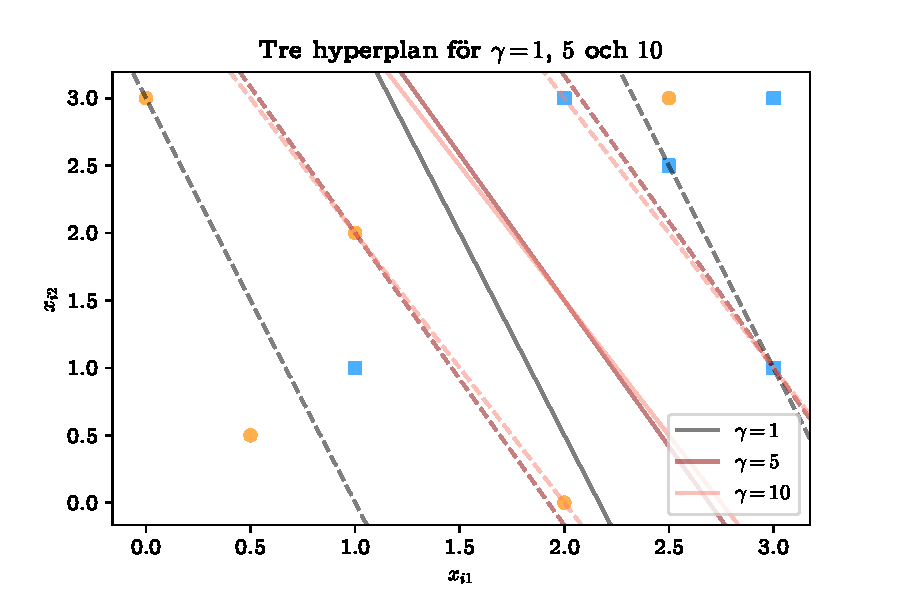
\includegraphics[width=0.8\linewidth, trim={0.5cm 2mm 0.5cm 6mm}, clip]{KandFigur2.pdf}
	\caption{\label{fig:mjukamarginaler}Löst exempel för linjärt oseparabelt data för 3 olika värden på $\gamma$. De streckade linjerna är marginalernas ränder.}
\end{figure}
Låt observationsparen $\left(\mathbf{x}_i,~y_i\right)$ vara sådana som i figur \ref{fig:mjukamarginaler} där blåa rutor är klassen $y_i=1$ och orangea cirklar är klassen $y_i=-1$. Axlarna motsvarar här $\mathbf{x}_i$:s första respektive andra komponenter. Klart är här att observationsparen inte är linjärt separabla men det verkar som att en punkt från vardera klassen kanske mätts fel. För att bestämma en klassificeringsregel används separerande hyperplan med mjuka marginaler för 3 olika värden på $\gamma$. Funktionen \texttt{SVC} med \texttt{kernel='linear'} från paketet \texttt{sklearn} \cite{sklearn} användes för att beräkna hyperplanen.

Observera hur parametern $\gamma$ påverkar lösningen. Ju mindre $\gamma$ är desto större är marginalerna vilket betyder att flera punkter används som stödvektorer.
\end{ex}
\begin{ex}\label{ex:olinjär}
\begin{figure}[h]
	\centering
	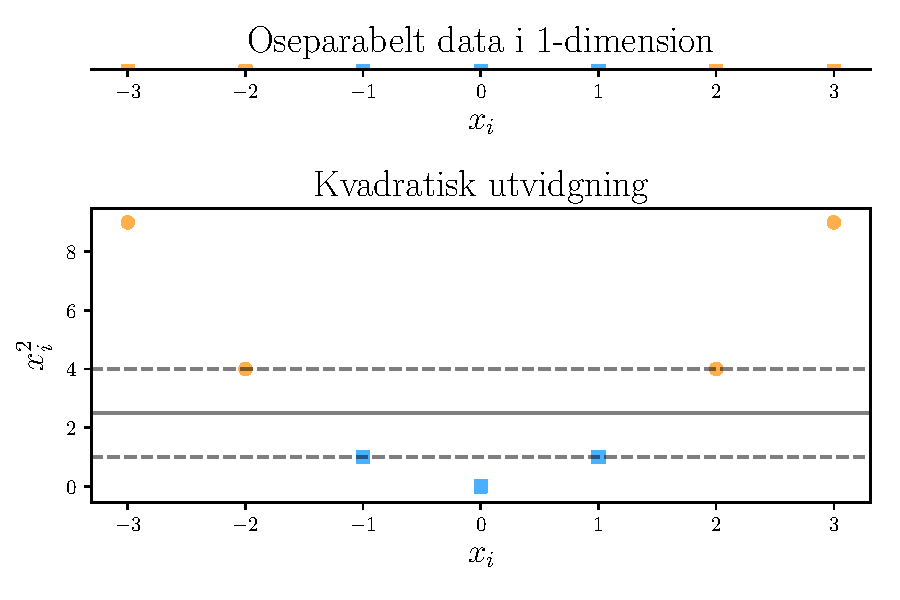
\includegraphics[width=0.8\linewidth, trim={0.5cm 4mm -5mm 4mm}, clip]{KandFigur3.pdf}
	\caption{\label{fig:kvadratisk}En lösning med optimala separerande hyperplan och kvadratisk utvidgning där endast hyperplan med mjuka marginaler inte hade fungerat.}
\end{figure}
Låt $\mathbf{x}_i\in\mathbb{R}$ och observationsparen $\left(\mathbf{x}_i,~y_i\right)$ vara sådana att klassen $y_i=1$ befinner sig mitt i klassen $y_i=-1$, situationen finns illustrerad överst i figur \ref{fig:kvadratisk}. Klart är att observationsparen är linjärt oseparabla men nu kan inte heller separerande hyperplan med mjuka marginaler ge vettiga lösningar. Istället kan man lägga till en dimension och definiera att $\mathbf{x}_i\in\mathbb{R}^2$ och $\mathbf{x}_{i2} = \mathbf{x}_{i1}^2$.
Då får man situationen som illustreras nederst i figur \ref{fig:kvadratisk} och observationsparen är nu linjärt separabla. Det optimala separerande hyperplanet bestämdes med hjälp av \texttt{sklearn}:s metod \texttt{SVC} med \texttt{kernel='linear'} och \texttt{C=1000} \cite{sklearn}.

Moralen är att hyperplan med mjuka marginaler inte alltid räcker till utan flera verktyg behövs. Ett sådant verktyg är olinjära utvidgningar av det ursprungliga rummet $\mathbf{x}_i\in \mathbb{R}^p$ till ett större rum där det kan vara enklare att hitta vettiga klassificeringsregler.
\end{ex}
%\FloatBarrier
\chapter{Reproducerande kärnor}
Exempel \ref{ex:olinjär} antyder att det kunde vara en bra idé att utvidga observationerna $\mathbf{x}_i$ med olinjära faktorer, frågan är bara hur detta görs bäst. I exemplet bildades andra gradens polynom för varje observation $\bfx_i$ så att de nya observationerna $\bfx_i'$ blev $\left[\bfx_i, \bfx_i^2\right]^\intercal$. Att räkna ut de nya $\bfx_i'$:na kommer då att kräva $N$ multiplikationer (kvadrering av $\bfx_i$); att bilda tredje gradens polynom hade krävt $2N$ multiplikationer och att bilda $n$:te gradens polynom hade tagit $nN$ multiplikationer. Efter utvidgningen löstes optimeringsproblemet 
\begin{equation*}
\begin{aligned}
\operatornamewithlimits{min}_{\bfbeta, \beta_0} & & &\frac{1}{2}\left\|\bfbeta
\right\|_2^2\\
\text{så att} & & &y_i\left(\inner{\bfx_i'}{\bfbeta}_2+\beta_0\right)\geq 1,\quad i=1,~\dots,~N
\end{aligned}
\end{equation*}
där $\bfbeta$ nu är en 2-dimensionell vektor. För att lösa ovanstående optimeringsproblem undersöks det duala Lagrangeproblemet
\begin{equation*}
		L_D= \sum_{i=1}^{N}\lambda_i - \frac{1}{2}\sum_{i=1}^{N}\sum_{j=1}^{N}\lambda_i\lambda_jy_iy_j\inner{\bfx_i'}{\bfx_j'}_2
\end{equation*}
där den sista dubbelsumman kan representeras som en matrismultiplikation:
\begin{equation*}
	\boldsymbol{\lambda}^\intercal\mathbf{K}\boldsymbol{\lambda}
\end{equation*}
där $\boldsymbol{\lambda}$ är en vektor bestående av värdena på $y_i\lambda_i$ och matrisen $\mathbf{K}$ är symmetrisk och har värdena $\mathbf{K}_{ij}=\inner{\bfx_i'}{\bfx_j'}_2$. För att räkna ut matrisen räknas inreprodukten $\inner{\bfx_i'}{\bfx_j'}_2$ ut för alla kombinationer men eftersom inreprodukten är symmetrisk måste inte elementen under diagonalen beräknas. Inreprodukten tar 3 operationer i anspråk, 2 för att multiplicera $\bfx_i'$ och $\bfx_j'$:s komponenter komponentvis och 1 för att summera. Inreprodukten måste räknas ut $\frac{N(N+1)}{2}$ gånger (se figur \ref{fig:comb}) så totalt måste en dator genomföra åtminstone $N$ + $3\frac{N(N+1)}{2}$ operationer före optimeringsproblemet kan börja lösas.
\begin{figure}[h]
	\centering
	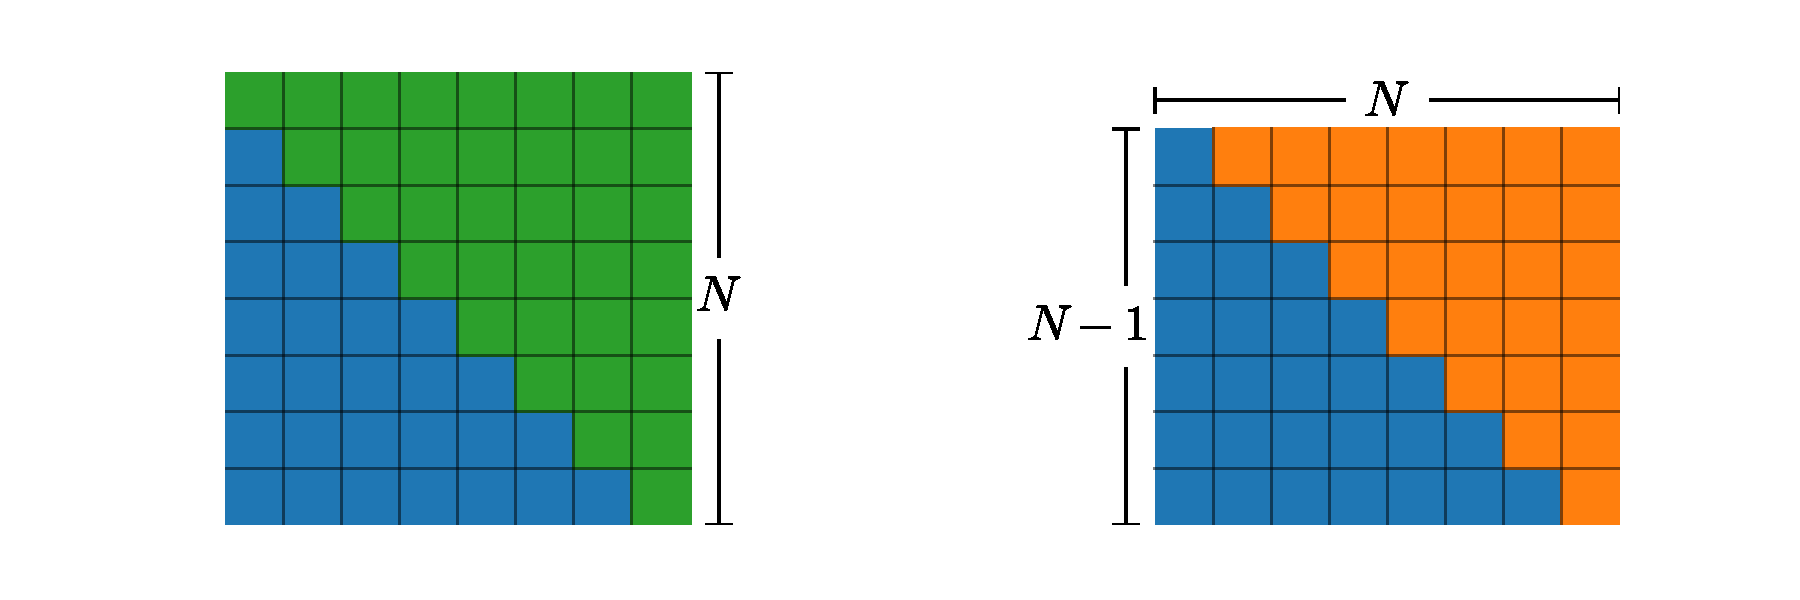
\includegraphics[width=0.8\linewidth, trim={3.5cm 11mm 2.7cm 11mm}, clip]{KandFigur5.pdf}
	\caption{\label{fig:comb}Visuellt bevis för hur många gånger man måste räkna ut inreprodukten $\inner{\bfx_i}{\bfx_j}_\hil$ där $i,~j=1,~\dots,~N$. Svaret blir $N^2-\frac{N(N-1)}{2}$ det vill säga antalet rutor i en $N\times N$ kvadrat minus antalet rutor under diagonalen som räknas till höger. Svaret ger antalet gröna rutor.}
\end{figure}

Hade man bildat $n$:te gradens polynom hade antalet operationer varit $nN$ för att räkna ut de nya observationerna och $(n+n-1)\frac{N(N+1)}{2}$ operationer för matrisen. Dessutom måste inreprodukten $\inner{\bfx_i'}{\bfbeta}_n$ räknas ut flera gånger när problemet löses.

Dimensionen på det ursprungliga rummet har inte ännu tagits i beaktande, i exempel \ref{ex:olinjär} var dimensionen 1 men vad händer om dimensionen är 2 eller 3? Eller kanske man har $16\times16$ pixlar stora bilder. Det visar sig att om den ursprungliga dimensionen $p$ är stor så får till och med enkla utvidgningar en mycket stor dimension $P$ vilket gör det arbetsamt att räkna ut inreprodukten $\inner{\bfx_i'}{\bfx_j'}_P$. Om man till exempel vill samla alla monom\footnote{Till exempel $\bfx_{i1}\bfx_{i2}\bfx_{i3}^2$ är ett monom av graden 5 medan  $\bfx_{i1}\bfx_{i2}\bfx_{i3}$ inte är det och inte $\bfx_{i1}\bfx_{i2}\bfx_{i3}^4$ heller.} av graden 5 för en $16\times16$ pixlar stor bild blir dimensionen nästan $10^{10}$ \cite{LearningKernels}.

Man kan dra slutsatsen att det borde finnas någon möjlighet att effektivera beräkningarna vilket visar sig vara sant. Istället för att först göra utvidgningarna kan man byta ut inreprodukten mot en annan funktion med vissa egenskaper. För exempel \ref{ex:olinjär} skulle den funktionen se ut på följande sätt:
	
	Betrakta funktionen $\phi:\left[\bfx\right]\longmapsto \left[\bfx^2,\sqrt{2}\bfx, 1\right]^\intercal$ där $\bfx\in\mathbb{R}$, denna funktion motsvarar den olinjära utvidgningen i exempel \ref{ex:olinjär}. Följande inreprodukt mellan två observationer $\mathbf{x}_1$ och $\mathbf{x}_2$ ska beräknas:
	\begin{align*}
	\left\langle \phi\left(\mathbf{x}_1\right), \phi\left(\mathbf{x}_2\right) \right\rangle_3 &= \bfx_1^2\bfx_2^2 + 2\bfx_1\bfx_2 + 1\\
	&= \langle \bfx_1, \bfx_2 \rangle_1^2 + 2\langle \bfx_1, \bfx_2 \rangle_1 + 1\\
	&= \left(\langle\bfx_1, \bfx_2 \rangle_1 + 1\right)^2 = k\left(\bfx_1, \bfx_2\right)
	\end{align*}
	där $\langle \cdot, \cdot \rangle_p$ är den vanliga inreprodukten i $\mathbb{R}^p$. Man byter alltså ut inreprodukten $\inner{\phi\left(\bfx_i\right)}{\phi\left(\bfx_j\right)}_3$ mot funktionen $k\left(\bfx_i, \bfx_j\right)=\left(\langle\bfx_1, \bfx_2 \rangle_1 + 1\right)^2$ när man löser optimeringsproblemet. I det här fallet gör man inga större besparingar när man räknar ut matrisen $\mathbf{K}$, eftersom inreprodukten $\inner{[\bfx_i^2, \bfx_i]^\intercal}{[\bfx_j^2, \bfx_j]^\intercal}_2$ endast kräver 3 operationer att beräkna (här används inreprodukten i $\mathbb{R}^2$  eftersom den sista komponenten i $\phi(\bfx)$ är konstant det vill säga onödig), lika många som funktionen $k$. Ifall man hade använt femte gradens polynom hade funktionen $k\left(\bfx_i, \bfx_j\right)=\left(\langle\bfx_1, \bfx_2 \rangle_1 + 1\right)^5$ krävt mellan 3 och 5 operationer att beräkna (beroende på hur exponentiering är implementerat\footnote{Antalet operationer blir 3 ifall datorn kan räkna ut $a^5$ med en operation, annars är $a^5=a^2a^2a$ där man inte behöver räkna ut $a^2$ två gånger och antalet operationer blir 5.}) medan inreprodukten $\inner{\cdot}{\cdot}_4$ kräver 7 operationer att räkna.
	
	Man behöver dessutom inte på förhand räkna ut de nya komponenterna för alla observationer och sparar således in $2N$ operationer i detta fall. För mera realistiska exempel med större dimensioner sparar man ofta mycket mera tid.

Funktioner $k\left(\bfx_1, \bfx_2\right)$ som kan uttryckas som en inreprodukt av en funktion $\phi$ evaluerad i två olika punkter $\bfx_1$ och $\bfx_2$ brukar kallas \emph{kärnor} och studerades först av David Hilbert \cite{Hilbert} i samband med studien av integraloperatorn $T_k f\left(x\right)=\int_{X}k\left(x_1, x_2\right)f\left(x_2\right)\,dx_2$ där funktionen $k$ är operatorn $T_k$:s kärna \cite{LearningKernels}.


%\section{Grundläggande teori}
%Först några grundläggande definitioner angående \emph{Hilbertrum}, $\mathcal{H}$, det vill säga \emph{fullständiga} vektorrum $X$ försedda med en \emph{inreprodukt} $\langle \cdot , \cdot \rangle$.
%
%\begin{defi}\label{def:inreprodukt}
%En \emph{inreprodukt} är en funktion $\langle \cdot , \cdot \rangle: X\times X \longmapsto \mathbb{R}$ sådan att, för alla $\mathbf{x},~\mathbf{y},~\mathbf{z}~\in X$ och alla $\lambda \in \mathbb{R}$, gäller:
%\begin{enumerate}
%\item $\inprod{x}{y} = \inprod{y}{x}$
%\item $\langle \lambda \mathbf{x}, \mathbf{y}\rangle = \lambda \inprod{x}{y}$
%\item $\inprod{x+y}{z} =\inprod{x}{z} + \inprod{y}{z}$
%\item $\inprod{x}{x} \geq 0$ där likhet gäller om och endast om $\mathbf{x} = \mathbf{0}$. 
%\end{enumerate}
%\end{defi}
%\begin{defi}
%Ett inreproduktrum $X$ är \emph{fullständigt} om varje Cauchyföljd $\mathbf{x}_n$ konvergerar (med avseende på normen inducerad av inreprodukten) till en punkt $\mathbf{x}$ i $X$.
%\end{defi}

%\begin{rem}
%Dimensionen på vektorrummet $X$ nämns inte i definitionen för inreprodukten och därför kan Hilbertrum även vara oändligtdimensionella. Många av de bekanta egenskaperna för ändligtdimensionella inreproduktrum gäller även för oändligtdimensionella inreproduktrum, till exempel är två vektorer $\mathbf{x}, ~\mathbf{y}$ ortogonala ifall $\inprod{x}{y}_\hil=0$, även om det kan vara svårt att visualisera för oändligtdimensionella rum.
%\end{rem}
%På tal om ortogonalitet så vore det behändigt att ha någon parallell till de ändligtdimensionella vektorrummens koordinatsystem och basvektorer. Det visar sig att inte alla Hilbertrum har en motsvarighet till basvektorer men ifall man kräver att rummet är \emph{separabelt} så existerar en ortonormal följd vektorer $\mathbf{e}_i$ sådan att för varje vektor $\mathbf{x}\in \mathcal{H}$  gäller \cite{Young}: %TODO	Definition på separabelt eller källa
%\begin{equation*}
%	\mathbf{x}=\sum_{i=1}^{\infty}\left\langle \mathbf{x}, \mathbf{e}_i \right\rangle_\hil \mathbf{e}_i
%\end{equation*}
%där vektorerna $\mathbf{e}_i$ agerar bas och koefficienten $\left\langle \mathbf{x}, \mathbf{e}_i \right\rangle_\hil$ kallas den $i$:te Fourierkoefficienten med avseende på basen $\mathbf{e}_i,$ $i=1,2,3,\dots$. I fortsättningen behandlas bara separabla Hilbertrum, så att varje vektor $\mathbf{x}$ kan skrivas som en linjär kombination av basvektorerna.

%Elementen i Hilbertrummen kan också ha många olika former, till exempel de $d$-dimensionella vektorerna med den vanliga inreprodukten $\left\langle \mathbf{x}, \mathbf{y} \right\rangle = \mathbf{x}^\intercal\mathbf{y}$ som hittills behandlats. Man kan även tillåta att elementen är funktioner, till exempel på intervallet $\left[a,b\right]$, då brukar inreprodukten definieras som
%\begin{equation*}
%	\left\langle f, g \right\rangle=\int_{a}^{b}f\left(x\right)g\left(x\right) dx,
%\end{equation*}
%men man måste dessutom kräva att normen $\left\|f\right\| = \left(\int_{a}^{b}f\left(x\right)^2dx\right)^{\frac{1}{2}}$ är ändlig för alla funktioner i rummet.

%Speciellt när det kommer till Hilbertrum med funktioner som element, så kallade \emph{funktionsrum}, så behandlar man \emph{funktionaler} istället för funktioner för att undvika förvirring.
%\begin{defi}
%	En \emph{funktional} $\mathcal{F}$ är en reellvärd funktion som tar en annan funktion $f$ som argument, det vill säga
%	\begin{equation*}
%		\mathcal{F}: \mathcal{H} \longmapsto \mathbb{R}
%	\end{equation*}
%	där elementen i Hilbertrummet $\mathcal{H}$ är funktioner.
%\end{defi}
%
%En funktional är linjär om följande gäller:
%\begin{equation*}
%	\mathcal{F}\left(\lambda f+g\right) = \lambda\mathcal{F}\left(f\right) + \mathcal{F}\left(g\right),
%\end{equation*}
%för alla $f$, $g$ $\in \mathcal{H}$, $\lambda \in \mathbb{R}$ och \emph{begränsad} om följande gäller:
%\begin{equation*}
%	\sup \left\{\left| \mathcal{F}\left(u\right) \right| : u\in\mathcal{H},~\left\| u \right\|_{\mathcal{H}} \leq 1 \right\} < \infty
%\end{equation*}
%där $\left\| \cdot \right\|_ \mathcal{H}$ är den inducerade normen i Hilbertrummet $\mathcal{H}$.
%
%Dessutom gäller att linjära funktionaler är begränsade om och endast om de är kontinuerliga. Det gäller även att funktionaler är kontinuerliga om och endast om de är kontinuerliga i 0 \cite{Young}.
%
%Följande sats ger ett sätt att karaktärisera varje begränsad linjär funktional $\mathcal{F}$ som en inreprodukt.
%
%\begin{thm}[Riesz-Fréchets representations sats \cite{Young}]
%	För varje begränsad linjär funktional på ett Hilbertrum $\mathcal{H}$, $\mathcal{F}: \mathcal{H} \longmapsto \mathbb{R}$, existerar ett unikt $v\in\mathcal{H}$ sådant att
%	\begin{equation}
%		\mathcal{F}\left(u\right)=\left\langle u, v\right\rangle_\mathcal{H}\quad \text{för alla }u\in\mathcal{H}, %TODO	Inte för alla?
%	\end{equation}
%	där $\left\langle \cdot, \cdot\right\rangle_\mathcal{H}$ betecknar inreprodukten i Hilbertrummet $\mathcal{H}$.\\
%	Dessutom gäller att $\left\| v \right\|_\mathcal{H}=\left\| \mathcal{F}\right\|_O$ där $\left\| \cdot \right\|_\mathcal{H}$ är den inducerade normen och $\left\|\cdot\right\|_O$ är operatornormen \begin{equation*}
%	\left\|\mathcal{F}\right\|_O:=\sup_{u\in\mathcal{H},\left\|u\right\|_\mathcal{H}\leq 1}\left|\mathcal{F}\left(u\right)\right|.
%	\end{equation*}
%\end{thm}
%\begin{proof}
%	Nedan följer en översikt av beviset i \cite{Young}.
%	
%	Ifall $\mathcal{F}$ är funktionalen som avbildar varje element $u\in\mathcal{H}$ på 0 så är satsen bevisad genom att man väljer $v=0$. 
%	
%	Antag att det existerar åtminstone ett $u\in\mathcal{H}$ sådant att $\mathcal{F}\left(u\right)\neq0$. Då kan man dela upp $\mathcal{H}$ i två delar,
%	\begin{equation*}
%		\mathcal{M} = \left\{u\in\mathcal{H}:\mathcal{F}\left(u\right)=0\right\}
%	\end{equation*}
%	och
%	\begin{equation*}
%		\mathcal{M}^\perp = \left\{u\in\mathcal{H}: \left\langle u,w \right\rangle=0\text{ för alla }w \in \mathcal{M}\right\},
%	\end{equation*}
%	det vill säga $\mathcal{M}^\perp$ är det \emph{ortogonala komplementet} till $\mathcal{M}$.
%	Då gäller att varje element $w_0\in \mathcal{H}$ kan skrivas som summan $w_0 = w_1 + w_2$ där $w_1\in\mathcal{M}$ och $w_2\in \mathcal{M}^\perp$ (Sats 4.24 i \cite{Young}). Lineariteten av $\mathcal{F}$ ger då att $\mathcal{F}\left(w_0\right)=\mathcal{F}\left(w_1\right)+\mathcal{F}\left(w_2\right)=\mathcal{F}\left(w_2\right)$, på grund av detta och antagandet att det existerar ett $w_0\in\mathcal{H}$ sådant att $\mathcal{F}\left(w_0\right)\neq0$ måste det finnas åtminstone ett element $w_2 \neq 0$ i $\mathcal{M}^\perp$. Välj $x:= \frac{w_2}{\mathcal{F}\left(w_2\right)}$, då är $\mathcal{F}\left(x\right)=\mathcal{F}\left(\frac{1}{\mathcal{F}\left(w_2\right)}w_2\right)=\frac{\mathcal{F}\left(w_2\right)}{\mathcal{F}\left(w_2\right)}=1$ och $x\in\mathcal{M}^\perp$.
%	För varje element $u\in\mathcal{H}$ kan man då skriva
%	\begin{equation*}
%		u=\underbrace{\left(u-\mathcal{F}\left(u\right)x \right)}_{\in\mathcal{M}} + \underbrace{\mathcal{F}\left(u\right)x}_{\in \mathcal{M}^\perp}.
%	\end{equation*}
%	Om man sedan tar inreprodukten med $x$ på båda sidorna så får man
%	\begin{align*}
%		\left\langle u,x \right\rangle &= \underbrace{\left\langle u-\mathcal{F}\left(u\right)x ,x \right\rangle}_{=0} + \left\langle \mathcal{F}\left(u\right)x,x \right\rangle\\
%		&= \mathcal{F}\left(u\right)\langle x, x\rangle=\mathcal{F}\left(u\right)\|x\|^2
%	\end{align*}
%	eftersom $u-\mathcal{F}\left(u\right)x\in\mathcal{M}$ och $\langle w, x \rangle=\langle x,w\rangle=0$ för alla element $w\in \mathcal{M}$ då $x\in\mathcal{M}^\perp$. Om man då väljer $v=\frac{x}{\|x\|^2}$ får man att
%	\begin{align*}
%		\langle u,v \rangle &= \left\langle u , \frac{x}{\|x\|^2}\right\rangle= \frac{\langle u, x\rangle}{\|x\|^2}\\
%		&= \frac{\mathcal{F}\left(u\right)\|x\|^2}{\|x\|^2}\\
%		&= \mathcal{F}\left(u\right)
%	\end{align*}
%	och då är den första delen av satsen bevisade. Den andra delen är inte lika intressant i detta fall så beviset lämnas bort.
%\end{proof}

%\section{Reproducerande Kärnor}


\section{Kärnor som inreprodukter}

Ovanstående exempel motiverar studien samt definitionen av \emph{kärnor}:
\begin{defi}[Enligt \cite{LearningKernels}]\label{def:kärna}
	Givet en funktion $\phi: \mathbb{R}^p \longmapsto \mathbb{R}^P$ definieras \emph{kärnan} $k$ som funktionen $k\left(\bfx, \bfy\right) = \langle \phi \left(\bfx\right), \phi\left(\bfy\right) \rangle_P$ där $\bfx, \bfy \in \mathbb{R}^p$ och $\langle \cdot, \cdot \rangle_P$ är den vanliga inreprodukten i $\mathbb{R}^P$.
	Vidare om man fixerar ett $\bfy\in\mathbb{R}^p$ så betecknar vi $\Phi_{\bfy}\left(\bfx\right) = k\left(\bfx, \bfy\right)$ där $\bfx\in\mathbb{R}^p$.
\end{defi}
%Den sista delen i definition \ref{def:kärna} ger med andra ord att varje val av ett fixt $\bfy$ ger upphov till en reellvärd funktion $\Phi_{\bfy}$ av $\bfx$.

Givet en mängd observationer $\bfx_i\in\mathbb{R},~i=1,~\dots,~N$, samt den polynomiella kärnan $k\left(\bfx, \bfy\right):=\left(\langle \bfx, \bfy \rangle_1 + 1\right)^2 = \left(\bfx\bfy\right)^{2} + 2\bfx\bfy + 1$, kan man definiera ett vektorrum av funktioner genom
\begin{equation*}
	f\left(\bfx\right):=\sum_{i=1}^{N}\alpha_ik\left(\bfx, \bfx_i\right)\quad ,~\alpha_i\in\mathbb{R}.
\end{equation*}
Varje funktion $f\left(\bfx\right)$ är alltså en linjär kombination av funktionerna $\Phi_{\bfx_i}\left(\bfx\right)=k\left(\bfx,\bfx_i\right)$ där $\bfx_i,~i=1,~\dots,~N$ är fixerade. %TODO	Klumpigt formulerat

För en annan funktion $g\left(\bfx\right):=\sum_{j=1}^{m}\beta_jk\left(\bfx, \bfx_j\right)$ i samma vektorrum kan man definiera inreprodukten
\begin{equation}\label{eq:polykärnaprodukt}
	\langle f , g\rangle_k := \sum_{i=1}^{N}\sum_{j=1}^{N} \alpha_i \beta_j k\left(\bfx_i, \bfx_j\right).
\end{equation}
Definitionen för $\langle f, g \rangle_k$ innehåller samma koefficienter som de linjära kombinationer som definierar $f$ och $g$ men eftersom
\begin{equation}\label{eq:expansion1}
	\langle f, g \rangle_k = \sum_{i=1}^{N} \sum_{j=1}^{N} \alpha_i \beta_j k\left(\bfx_i, \bfx_j\right) = \sum_{i=1}^{N} \alpha_i \sum_{j=1}^{N}\beta_j k\left(\bfx_i, \bfx_j\right)=\sum_{i=1}^{N} \alpha_i g\left(\bfx_i\right)
\end{equation}
och
\begin{equation}\label{eq:expansion2}
\begin{aligned}
	\langle f, g \rangle_k &= \sum_{i=1}^{N} \sum_{j=1}^{N} \alpha_i \beta_j \left(\left(\bfx_i\bfx_j\right)^2 + 2\bfx_i\bfx_j+1\right)\\
	&= \sum_{j=1}^{N} \sum_{i=1}^{N} \alpha_i \beta_j \left(\left(\bfx_j\bfx_i\right)^2 + 2\bfx_j\bfx_i+1\right) = \sum_{j=1}^{N} \beta_j \sum_{i=1}^{N}\alpha_i k\left(\bfx_j, \bfx_i\right) \\
	&= \sum_{j=1}^{N} \beta_j f\left(\bfx_j\right)
\end{aligned}
\end{equation}
så beror inte summan på vilka linjära kombinationer man väljer för funktionerna $f$ och $g$ ifall de inte går att välja unikt. Som mellansteg visades även att $k\left(\bfx_i, \bfx_j\right)=k\left(\bfx_j, \bfx_i\right)$.

För att visa att $\langle f, g \rangle_k$ är en inreprodukt måste man kolla att alla villkor i definition \ref{def:inreprodukt} är uppfyllda:
\begin{enumerate}
	\item[\ref{IP1}] $\langle f, g \rangle_k=\langle g, f \rangle_k$:
	\begin{align*}
		\langle f, g \rangle_k = \sum_{i=1}^{N} \sum_{j=1}^{N} \alpha_i \beta_j k\left(\bfx_i, \bfx_j\right) \overset{(\ref{eq:expansion2})}{=} \sum_{j=1}^{N} \sum_{i=1}^{N}  \beta_j \alpha_i k\left(\bfx_j, \bfx_i\right) = \langle g, f \rangle_k
	\end{align*}
	där man kan kasta om summorna eftersom de är ändliga. \hfill \qedsymbol
	\item[\ref{IP2}] $\langle \lambda f, g \rangle_k=\lambda\langle f, g \rangle_k,~\lambda\in\mathbb{R}$:
	\begin{equation*}
	\pushQED{\qed}
		\langle \lambda f, g \rangle_k	\overset{\left(\ref{eq:expansion2}\right)}{=} \sum_{j=1}^{N} \beta_j \lambda f\left(\bfx_j\right) = \lambda \sum_{j=1}^{N} \beta_j f\left(\bfx_j\right) = \lambda\langle f, g \rangle_k \qedhere
		\popQED
	\end{equation*}
	\item[\ref{IP3}] $\langle f+h, g\rangle_k = \langle f, g\rangle_k + \langle h, g\rangle_k$:
	\begin{align*}
		\langle f+h, g \rangle_k \overset{(\ref{eq:expansion2})}{=} &\sum_{j=1}^{N} \beta_j \left(f\left(\bfx_j\right) + h\left(\bfx_j\right)\right)\\
		= &\sum_{j=1}^{N} \beta_j f\left(\bfx_j\right) + \sum_{j=1}^{N} \beta_j h\left(\bfx_j\right)\\
		= &\langle f, g\rangle_k + \langle h, g\rangle_k
	\end{align*}
	där även $h$ kan skrivas som en linjär kombination men beviset beror inte på vilken kombination man väljer. \hfill \qedsymbol
	\item[\ref{IP4}] $\langle f, f \rangle_k\geq0$:
	\begin{align*}
	\langle f, f \rangle_k &= \sum_{i=1}^{N}\sum_{j=1}^{N}\alpha_i\alpha_jk\left(\bfx_i, \bfx_j\right)
	= \sum_{i=1}^{N}\sum_{j=1}^{N}\alpha_i\alpha_j\left\langle\phi\left(\bfx_i\right),\phi\left(\bfx_j\right)\right\rangle_3\\
	&= \sum_{i=1}^{N}\alpha_i\sum_{j=1}^{N}\alpha_j\left\langle\phi\left(\bfx_j\right),\phi\left(\bfx_i\right)\right\rangle_3
	= \sum_{i=1}^{N}\alpha_i\left\langle\sum_{j=1}^{N}\alpha_j\phi\left(\bfx_j\right),\phi\left(\bfx_i\right)\right\rangle_3\\
	&= \sum_{i=1}^{N}\alpha_i\left\langle\phi\left(\bfx_i\right),\sum_{j=1}^{N}\alpha_j\phi\left(\bfx_j\right)\right\rangle_3
	= \left\langle\sum_{i=1}^{N}\alpha_i\phi\left(\bfx_i\right),\sum_{j=1}^{N}\alpha_j\phi\left(\bfx_j\right)\right\rangle_3\\
	&= \left\|\sum_{i=1}^{N}\alpha_i\phi\left(\bfx_i\right)\right\|_3^2\geq 0
	\end{align*}
	där likhet gäller om och endast om $\sum_{i=1}^{N}\alpha_i\phi\left(\bfx_i\right)=\mathbf{0}$.
	
	För
	\begin{equation*}
		f\left(\bfx\right)=\sum_{i=1}^{N}\alpha_i k\left(\bfx, \bfx_i\right) = \sum_{i=1}^{N}\alpha_i \left\langle\phi\left(\bfx\right), \phi\left(\bfx_i\right) \right\rangle_3 = \left\langle \phi\left(\bfx\right), \sum_{i=1}^{N}\alpha_i\phi\left(\bfx_i\right) \right\rangle_3
	\end{equation*}
	gäller då att om $\langle f, f \rangle_k = 0$ så är $\ \sum_{i=1}^{N}\alpha_i\phi\left(\bfx_i\right)=\mathbf{0}$ och då även
	\begin{equation*}
		f\left(\bfx\right) = \left\langle \phi\left(\bfx\right), \sum_{i=1}^{N}\alpha_i\phi\left(\bfx_i\right) \right\rangle_3 = \left\langle \phi\left(\bfx\right), \mathbf{0}\right\rangle_3=0.
	\end{equation*}
	Med andra ord är $\left\langle f,f\right\rangle\geq0$ där likhet gäller om och endast om $f\left(\bfx\right)=0$ för alla $\bfx$.
	\qquad \hfill \qedsymbol
	
%	För att visa att $\langle f, f\rangle = 0$ om och endast om $f=0$ det vill säga alla $\alpha_i, i=1,~\dots,~N$ krävs en motsvarighet till Cauchy-Scwharz olikheten men formulerad för kärnor det vill säga
%	\begin{thm}[Cauchy-Scwharz olikhet för kärnor \cite{LearningKernels}]\label{thm:cauchy}
%		För en \emph{positivt definit} kärna $k$ och $\bfx_1,~\bfx_2\in V$ där $V$ är något vektorrum gäller att
%		\begin{equation}
%		|k\left(\bfx_1,\bfx_2\right)|^2 \leq k\left(\bfx_1,\bfx_1\right) k\left(\bfx_2,\bfx_2\right)
%		\end{equation}
%	\end{thm}
%	\begin{proof}
%		Betrakta matrisen $\mathbf{K}$ med elementen $\mathbf{K}_{ij}=k\left(\bfx_1, \bfx_2\right)$. Eftersom $k$ är positivt definit är även $\mathbf{K}$ positivt definit alltså är alla egenvärden positivta och då även determinanten positivt \left(se till exempel \cite{Axler} eller nästan vilken bok om linjär algebra/matristeori som helst), det vill säga
%		\begin{equation*}
%			\mathbf{K}_{11} \mathbf{K}_{22} - \mathbf{K}_{12} \mathbf{K}_{21} \geq 0.
%		\end{equation*}
%		Då $\mathbf{K}_{ij} = k\left(\bfx_i, \bfx_j\right)$ är symmetrisk enligt (\ref{eq:expansion2}) så fås att
%		\begin{equation*}
%			\mathbf{K}_{11} \mathbf{K}_{22} \geq \left|\mathbf{K}_{12}\right|^2
%		\end{equation*}
%		alltså gäller
%		\begin{equation*}
%			k\left(\bfx_1,\bfx_1\right) k\left(\bfx_2,\bfx_2\right) \geq |k\left(\bfx_1,\bfx_2\right)|^2\qedhere
%		\end{equation*}
%	\end{proof}
%	För att visa att $\langle f, f \rangle_k=0$ om och endast om $f=0$, det vill säga alla $\alpha_i=0$, notera först att följande gäller
%	\begin{equation*}
%		\langle \Phi_{\bfx_k}, f\rangle_k = \langle k\left(\cdot, \bfx_i\right), f\rangle_k = \sum_{j=1}^{N}\sum_{i=1}^{N}\beta_j\alpha_i k\left(\bfx_j, \bfx_i\right)
%	\end{equation*}
%	där $\beta_j = 0$ om $j\neq k$ och $1$ om $j=k$, det vill säga
%	\begin{equation}\label{eq:reproducing1}
%		\langle \Phi_{\bfx_k}, f\rangle_k = \sum_{i=1}^{N}\alpha_i k\left(\bfx_k, \bfx_i\right) = f\left(\bfx_k\right).
%	\end{equation}
%	och speciellt fås att
%	\begin{equation*}
%		\langle \Phi_{\bfx_k}, \Phi_{\bfx_l} \rangle_k = \sum_{i=1}^{N}\sum_{j=1}^{N}\alpha_i\beta_jk\left(\bfx_i, \bfx_j\right)
%	\end{equation*}
%	där $\alpha_i=\beta_j=1$ endast om $i=k$ och $j=l$, $\alpha_i=\beta_j=0$ annars. Då fås
%	\begin{equation*}
%	\langle \Phi_{\bfx_k}, \Phi_{\bfx_l} \rangle_k = \alpha_k\beta_lk\left(\bfx_k,\bfx_l\right) = k\left(\bfx_k, \bfx_l\right).
%	\end{equation*}
%	Sats \ref{thm:cauchy} och ekvation (\ref{eq:reproducing1}) ger då
%	\begin{equation*}
%		|f\left(\bfx\right)|^2 = |\left\langle \Phi_{\bfx},f\right\rangle_k|^2 \leq k\left(\bfx, \bfx \right)\left\langle f, f \right\rangle_k
%	\end{equation*}

\end{enumerate}
Eftersom alla villkor i definition \ref{def:inreprodukt} är uppfyllda så definierar $\langle f, g\rangle_k:=\sum_{i=1}^{N}\sum_{j=1}^{N}\alpha_i\beta_jk\left(\bfx_i, \bfx_j\right)$ en inreprodukt. Här är $k\left(\bfx, \bfy\right)=\left(\langle \bfx, \bfy\rangle_1 + 1\right)^2= \left\langle \phi\left(\bfx\right),  \phi\left(\bfy\right)\right\rangle_3$ och $\phi\left(\bfx\right)=\left[\bfx^2, \sqrt{2}\bfx, 1 \right]^\intercal$. Om man dessutom kräver att alla Cauchyföljder konvergerar till en funktion i samma rum så har man ett Hilbertrum vilket betyder att allting i kapitel \ref{chap:hilbert} gäller även här.

I beviset användes egenskap (\ref{eq:expansion2}) flitigt. Det visar sig att det räcker med att kärnan $k$ är symmetrisk det vill säga $k\left(\bfx_i, \bfx_j\right)=k\left(\bfx_j, \bfx_i\right)$ som garanteras om kärnan kan definieras som den naturliga inreprodukten mellan någon funktion $\phi\left(\mathbf{x}\right)$ evaluerad i punkterna $\bfx_i$ och $\bfx_j$. Med andra ord kan man dra slutsatsen att följande sats gäller:
\begin{thm}[Enligt \cite{LearningKernels}]\label{thm:kärnainreprodukt}
	För en kärna $k$ definierad som i definition \ref{def:kärna}, det vill säga $k\left(\bfx, \bfy\right)=\langle \phi\left(\bfx\right), \phi\left(\bfy\right)\rangle_P$ där $\phi\left(\cdot\right)$ är någon utvidgning, är rummet av funktioner definierade genom $f\left(\bfx\right) = \sum_{i=1}^{N}\alpha_ik\left(\bfx, \bfx_i\right)$ med inreprodukten $\langle f, g\rangle_k = \sum_{i=1}^{N}\sum_{j=1}^{N} \alpha_i\beta_jk\left(\bfx_i, \bfx_j\right)$ ett inreproduktrum.
\end{thm}
Dessutom fås även följande korollarium:
\begin{cor}[Enligt \cite{LearningKernels}]\label{cor:kärnahilbert}
	Om dessutom alla Cauchyföljder konvergerar till en funktion i samma rum, med avseende på normen inducerad av inreprodukten $\langle f, g\rangle_k$, så är rummet ett Hilbertrum.
\end{cor}

Nu kan man fundera på om kärnan $k$ måste vara definierad genom en inreprodukt, det kan ju hända att även andra funktioner $X \times X \longmapsto \mathbb{R}$ ger upphov till ett liknande Hilbertrum. Som sagt så garanterar inreprodukten att $k$ är symmetrisk men det finns säkert symmetriska funktioner som inte kan definieras genom inreprodukter. På samma sätt så garanterade inreprodukten att egenskap \ref{IP4} uppfylldes men man kan istället genast kräva att
\begin{equation*}
	\langle f, f \rangle_k = \sum_{i=1}^{N}\sum_{j=1}^{N}\alpha_i\alpha_jk\left(\bfx_i, \bfx_j\right) \geq 0
\end{equation*}
med likhet om och endast om $f=0$. Detta krav kan skrivas om som en matrismultiplikation:
\begin{equation}\label{eq:positivtsemidefinit}
\langle f, f \rangle_k = \sum_{i=1}^{N}\sum_{j=1}^{N}\alpha_i\alpha_jk\left(\bfx_i, \bfx_j\right) = \boldsymbol{\alpha}^\intercal \mathbf{K} \boldsymbol{\alpha}\geq 0
\end{equation}
där $\boldsymbol{\alpha}$ är en vektor med elementen $\alpha_1,~\alpha_2,~\dots,~\alpha_N$ och $\mathbf{K}$ är matrisen med elementen $\mathbf{K}_{ij}=k\left(\bfx_i, \bfx_j\right)$. Matrisen $\mathbf{K}$ kallas Gram-matrisen och kravet i (\ref{eq:positivtsemidefinit}) brukar användas som definition på \emph{positivt semidefinithet} för en matris $\mathbf{K}$. En funktion $k\left(\bfx_i, \bfx_j\right)$ sägs vara positivt semidefinit om Gram matrisen $\mathbf{K}_{ij}=k\left(\bfx_i, \bfx_j\right)$ är positivt semidefinit för alla val av $\bfx_i,~\bfx_j$.
\newpage
\section{Kärnor som positivt semidefinita funktioner}

Ovan gavs en motivering för varför man borde utvidga definitionen av kärnor.
\begin{defi}[Enligt \cite{LearningKernels}]
	En kärna är en symmetrisk positivt semidefinit funktion $k: X \times X \longmapsto \mathbb{R}$.
\end{defi}

Med små modifikationer gäller då beviset för sats \ref{thm:kärnainreprodukt} och korollarium \ref{cor:kärnahilbert} även för följande sats och korollarium:
\begin{thm}[Enligt \cite{LearningKernels}]
	För en kärna det vill säga en symmetrisk positivt semidefinit funktion $k: X \times X \longmapsto \mathbb{R}$ är rummet med funktioner definierade genom $f\left(\bfx\right) = \sum_{i=1}^{N}\alpha_ik\left(\bfx, \bfx_i\right)$ och inreprodukten $\langle f, g\rangle_k = \sum_{i=1}^{N}\sum_{j=1}^{N} \alpha_i\beta_jk\left(\bfx_i, \bfx_j\right)$ ett inreproduktrum.
\end{thm}
\begin{cor}[Enligt \cite{LearningKernels}]
	Om dessutom alla Cauchyföljder konvergerar till en funktion i samma rum, med avseende på normen inducerad av inreprodukten $\langle f, g\rangle_k$, så är rummet ett Hilbertrum.
\end{cor}
Betrakta funktionen $\Phi_{\bfx_l}(\bfx):=k\left(\bfx, \bfx_l\right)$,  där $k\left(\bfx, \bfy\right)$ är en symmetrisk positivt semidefinit funktion.  Funktionen $\Phi_{\bfx_l}\!(\bfx)$ kan skrivas som $\sum_{j=1}^{N}\!\beta_jk\left(\bfx, \bfx_l\right)$ med $\beta_j=1$ om $j=l$, 0 annars, för att passa in i definitionen för inreprodukten $\inner{\cdot}{\cdot}_k$. För $\Phi_{\bfx_l}(\bfx)$ och en annan funktion $f\left(\bfx\right) = \sum_{i=1}^{N}\alpha_ik\left(\bfx, \bfx_i\right)$ gäller då att
	\begin{equation*}
		\langle \Phi_{\bfx_l}, f\rangle_k = \langle k\left(\cdot, \bfx_i\right), f\rangle_k = \sum_{j=1}^{N}\sum_{i=1}^{N}\beta_j\alpha_i k\left(\bfx_j, \bfx_i\right)
	\end{equation*}
	där $\beta_j = 0$ om $j\neq l$ och $1$ om $j=l$, det vill säga
	\begin{equation}\label{eq:reproducing1}
		\langle \Phi_{\bfx_l}, f\rangle_k = \sum_{i=1}^{N}\alpha_i k\left(\bfx_l, \bfx_i\right) = f\left(\bfx_l\right).
	\end{equation}
	Speciellt för en annan funktion $\Phi_{\bfx_h}(\bfx):=k\left(\bfx, \bfx_h\right)$ fås att
	\begin{equation*}
		\langle \Phi_{\bfx_l}, \Phi_{\bfx_h} \rangle_k = \sum_{i=1}^{N}\sum_{j=1}^{N}\alpha_i\beta_jk\left(\bfx_i, \bfx_j\right)
	\end{equation*}
	där $\alpha_i=\beta_j=1$ endast om $i=l$ och $j=h$, $\alpha_i=\beta_j=0$ annars. Då fås
	\begin{equation}\label{eq:reproducing2}
	\begin{aligned}
	\langle \Phi_{\bfx_l}, \Phi_{\bfx_h} \rangle_k &= \inner{k\left(\cdot, \bfx_l\right)}{k\left(\cdot, \bfx_h\right)}_k\\ &= \alpha_l\beta_hk\left(\bfx_l, \bfx_h\right)\\&= k\left(\bfx_l, \bfx_h\right).
	\end{aligned}
	\end{equation}
Tolkningen av ekvation (\ref{eq:reproducing1}) är att inreprodukten mellan en funktion $f$ och $k\left(\cdot, \bfx_i\right)$ är samma sak som evaluering av funktionen $f$ i punkten $\bfx_i$ men $\bfx_i$ måste vara en av de punkterna som man byggde upp inreprodukten av.

För ekvation (\ref{eq:reproducing2}) är tolkningen att även om $k\left(\bfx_l, \bfx_h\right)$ inte är definierad genom en inreprodukt så kan $k$ tolkas som en inreprodukt i något (olinjärt) rum. De här två egenskaperna är orsaken till att man pratar om \emph{reproducerande} kärnor, den första ekvationen brukar också ibland användas som definitionen på en reproducerande kärna. Med andra ord borde man givet en symmetrisk positivt semidefinit funktion $k$ kunna skriva den som en inreprodukt i något rum, nedan följer ett exempel som på samma gång visar en av de största fördelarna med att använda kärnor istället för att räkna ut en olinjär utvidgning på förhand.

\begin{ex}
	Låt $\bfx_i,~\bfx_j\in\mathbb{R}$ och betrakta funktionen
	\begin{align*}
		k\left(\bfx_i, \bfx_j\right)&=e^{-\frac{\left\| \bfx_i-\bfx_j\right\|_1^2}{2\sigma^2}}\\&=e^{-\frac{\inner{\bfx_i-\bfx_j}{\bfx_i-\bfx_j}_1}{2\sigma^2}}\\
		&=e^{-\frac{\bfx_i^2+\bfx_j^2-2\bfx_i\bfx_j}{2\sigma^2}}\\&=e^{-\frac{\bfx_i^2+\bfx_j^2}{2\sigma^2}}\cdot e^{\frac{2\bfx_i\bfx_j}{2\sigma^2}}\\
		&= e^{-\left(\frac{\bfx_i}{\sqrt{2}\sigma}\right)^2}\cdot e^{-\left(\frac{\bfx_j}{\sqrt{2}\sigma}\right)^2}\cdot e^{\frac{\bfx_i\bfx_j}{\sigma^2}}.
	\end{align*}
	Genom Taylorutvecklingen för $e^{z}$ fås
	\begin{align*}
		k\left(\bfx_i, \bfx_j\right)&= e^{-\left(\frac{\bfx_i}{\sqrt{2}\sigma}\right)^2}\cdot e^{-\left(\frac{\bfx_j}{\sqrt{2}\sigma}\right)^2}\cdot \sum_{n=0}^{\infty}\frac{\bfx_i^n\bfx_j^n}{n!}\\
		&= \sum_{n=0}^{\infty} \left(\frac{e^{-\left(\frac{\bfx_i}{\sqrt{2}\sigma}\right)^2} \bfx_i^n}{\sqrt{n!}}\right)\left(\frac{e^{-\left(\frac{\bfx_j}{\sqrt{2}\sigma}\right)^2} \bfx_j^n}{\sqrt{n!}}\right)\\
		&= \inner{\phi\left(\bfx_i\right)}{\phi\left(\bfx_j\right)}_{\ell^2}
	\end{align*}
	där $\inner{\bfx}{\bfy}_{\ell^2}$ är inreprodukten given av summan $\sum_{i=1}^{\infty}\bfx_i\bfy_i$ om den är ändlig. Här betecknar $\bfx_i,~\bfy_i$ de $i$:te komponenterna av de oändligtdimensionella vektorerna $\bfx$ och $\bfy$. Summan konvergerar om $\bfx$ och $\bfy$ tillhör Hilbertrummet $\ell^2$ det vill säga rummet av alla följder $\bfx$ för vilka summan $\sum_{i=1}^{\infty}\bfx_i^2=\inner{\bfx}{\bfx}_{\ell^2}=\left\|\bfx\right\|_{\ell^2}^2$ är ändlig, detta eftersom $\inner{\bfx}{\bfy}_{\ell^2}^2\leq\inner{\bfx}{\bfx}_{\ell^2}\inner{\bfy}{\bfy}_{\ell^2}<\infty$ enligt sats \ref{CauchySchwarz}.
	
	Kärnan $k\left(\bfx, \bfy\right)=e^{-\frac{\left\| \bfx-\bfy\right\|^2}{2\sigma^2}}$ kan med andra ord skrivas som inreprodukten $\inner{\phi\left(\bfx\right)}{\phi\left(\bfy\right)}_{\ell^2}$ i rummet som ges av utvidgningen
	\begin{equation*}
	\phi\left(\bfx\right)=\left[\frac{e^{-\left(\frac{\bfx}{\sqrt{2}\sigma}\right)^2} \bfx^0}{\sqrt{0!}}, \frac{e^{-\left(\frac{\bfx}{\sqrt{2}\sigma}\right)^2} \bfx^1}{\sqrt{1!}}, \frac{e^{-\left(\frac{\bfx}{\sqrt{2}\sigma}\right)^2} \bfx^2}{\sqrt{2!}}, \dots\right]^\intercal.
	\end{equation*}
	
	Implikationen är att motsvarande olinjära transformation skulle ge ett oändligtdimensionellt rum att jobba med om man gör transformationen direkt medan man genom kärnan $k$ implicit kan jobba i ett oändligtdimensionellt rum, något som inte hade varit möjligt om man försökte operera med vanliga inreprodukter på det utvidgade rummet.
\end{ex}



\chapter{Avslutning}
Det finns också andra sätt att härleda stödvektormaskinernas optimeringsproblem, till exempel genom Tikhonov-regularisation. Andra härledningar kan ge nya insikter, till exempel kan man se stödvektormaskiner som en medlem i en större grupp av modeller innefattande bland annat spline-modeller \cite{ESL}. Med några små förändringar kan man också använda stödvektormaskiner för regression. Man kan också ändra på objektfunktionen för att uppmuntra lösningarna att ha vissa egenskaper, till exempel bara vara olika 0 i ett fåtal dimensioner (gles) \cite{LearningKernels}.

Stödvektormaskinerna utvecklades under 1990-talet ungefär på samma gång som Vapnik-Chervonenkis teorin där man försöker karaktärisera när och varför metoder inom maskininlärning och statistik generaliserar väl till nya observationer \cite{VC}. Vapnik-Chervonenkis teorin kan ses som ett försök att möjliggöra till exempel analys av konfidensintervall för mera komplicerade algoritmer än linjär regression. För stödvektormaskiner med mjuka marginaler och kärnor forskas det ännu i vilka teoretiska gränser man kan ge för generalisering till ny data \cite{theoretical}.

För att algoritmerna skall generalisera så väl som möjligt måste man ofta bestämma olika parametrar som inte kan lösas genom vanlig optimering. Till exempel måste parametern $\gamma$ och kärnan bestämmas på något sätt. Oftast görs detta genom att man löser algoritmen för till exempel 80 \% av observationerna med olika val av kärna och $\gamma$ för att sedan välja den kombination som fungerar bäst på de resterande 20 \%:en av observationerna \cite{ESL}.

De reproducerande kärnorna kan också användas för att göra andra algoritmer mera flexibla, det huvudsakliga kravet är att observationerna ska förekomma endast i inreprodukter \cite{ESL, LearningKernels}. Till exempel finns det versioner av principalkomponentsanalys (principal component analysis, PCA) och linjär diskriminantanalys (linear discriminant analysis, LDA) som gjorts olinjära med hjälp av reproducerande kärnor \cite{ESL}.

\bibliographystyle{sweplain}
\bibliography{bibliografi}
\end{document}
